% =====================================================================
%  Local Curvature, Trace Periods, and Galois Covers of Black-Hole Horizons
%  PREPRINT v2.1 --- 13 July 2026
%  Author: William Lloyd
%  Unified sequential manuscript (not a source dump).
%  Mathematical sources: local curvature calculus v1.0; DBP Landen--Trace
%  v1.1; Galois horizon cover v1.0 --- rewritten as one narrative.
% =====================================================================
\documentclass[11pt,a4paper]{article}

\usepackage[margin=1.05in]{geometry}
\usepackage{amsmath,amssymb,amsthm,mathtools}
\usepackage[T1]{fontenc}
\usepackage[utf8]{inputenc}
\usepackage{lmodern}
\usepackage{microtype}
\usepackage{booktabs}
\usepackage{array}
\usepackage{tabularx}
\usepackage{enumitem}
\usepackage{graphicx}
\usepackage{float}
\usepackage{xcolor}
\usepackage{tikz}
\usetikzlibrary{arrows.meta,positioning,fit,calc}
\usepackage[colorlinks=true,linkcolor=blue,citecolor=blue,urlcolor=blue]{hyperref}

\hypersetup{
  pdftitle={Local Curvature, Trace Periods, and Galois Covers of Black-Hole Horizons},
  pdfauthor={William Lloyd},
  pdfsubject={Preprint v2.1}
}

\setlist[itemize]{leftmargin=1.5em,itemsep=0.25em,topsep=0.35em}
\setlist[enumerate]{leftmargin=1.5em,itemsep=0.25em,topsep=0.35em}
\setlength{\parskip}{0.35em}
\setlength{\parindent}{1.2em}

\newtheorem{theorem}{Theorem}[section]
\newtheorem{proposition}[theorem]{Proposition}
\newtheorem{lemma}[theorem]{Lemma}
\newtheorem{corollary}[theorem]{Corollary}
\theoremstyle{definition}
\newtheorem{definition}[theorem]{Definition}
\theoremstyle{remark}
\newtheorem{remark}[theorem]{Remark}
\newtheorem{observation}[theorem]{Observation}
\newtheorem{example}[theorem]{Example}

\newcommand{\Q}{\mathbb{Q}}
\newcommand{\ZZ}{\mathbb{Z}}
\newcommand{\RR}{\mathbb{R}}
\newcommand{\NN}{\mathbb{N}}
\newcommand{\FF}{\mathbf{F}}
\newcommand{\disc}{\Delta}
\newcommand{\Gal}{\mathrm{Gal}}
\newcommand{\Res}{\mathrm{Res}}
\newcommand{\wrp}{\mathop{\mathrm{wr}}}
\newcommand{\ord}{\operatorname{ord}}
\newcommand{\CPV}{\operatorname{CPV}}
\newcommand{\Resop}{\operatorname{Res}}
% Notation discipline:
%   \Theta  = descended DBP trace differential on E_{128}
%   \vartheta = Galois-odd ST datum on a horizon branch
%   \mathcal{D} = local transverse first-drift sum (never called Theta)

\title{\textbf{Local Curvature, Trace Periods, and\\
Galois Covers of Black-Hole Horizons}\\[8pt]
\large Valuations, Landen--Trace reductions, and the\\
degree-$20$ entropy crown\\[10pt]
\normalsize\fbox{PREPRINT v2.1 --- 13 July 2026}}
\author{William Lloyd\\
\small Lloyd Geometric Diagnostics Pty Ltd, Coffs Harbour, NSW, Australia}
\date{}

\begin{document}
\maketitle

% =====================================================================
\begin{abstract}
Multi-horizon black-hole thermodynamics is organised here at three successive
scales. Locally, near normal-crossing collapses of thermodynamic coordinates,
diagonal inverse-channel metrics admit an exact directional decomposition of
scalar curvature. A master quadratic form on the metric valuation matrix
controls normal-vertex coefficients and yields the generic order-three and
parity-fixed order-four face laws, proper-distance rates, and a complete
cancellation hierarchy in arbitrary codimension. At the period scale, the
complementary complete integrals that arise from those channels reduce by
explicit degree-two isogenies to a common elliptic curve \(E_{128}\): each
differential splits into a non-torsion third-kind trace form \(\Theta\) and an
elementary logarithmic anti-translation term, with exact primary and dual
anti-periods. Globally, the horizon entropy pair is a Galois cover of the
observables. For Kerr--Newman the cover is quadratic and the left/right
dictionary is its \(\ZZ/2\) grading; at four charges the seed-mass fiber is an
\(S_5\) quintic, so Abel--Ruffini obstructs radical expressions for mass and
entropy while the area product remains rational. Above the quintic the static
ordered-horizon field has degree \(20\) and normal closure \(C_2^2\wrp S_5\);
rotation lifts to \(C_2^3\wrp S_5\). The paper is written as a single sequential
argument from local valuations through period reduction to Galois descent.
\end{abstract}

\tableofcontents
\newpage

% =====================================================================
\section{Introduction}
\label{sec:intro}
% =====================================================================

The thermodynamics of multi-horizon black holes is usually presented as a
collection of exact identities: sector entropies and temperatures, first laws
on both horizons, negative inner temperatures, universal area products, and
hidden-conformal data
\cite{CL1,CL2,CGLP2018,AH,CGP2011,CR2012,CMS,WangLiu,ChenLong4Q}. Those
identities are almost always derived by writing the outer and inner entropies
\(S_\pm\) explicitly in an auxiliary solution-generating frame---a seed mass
\(m\) and boost parameters \(\delta_i\) \cite{CY,Std4Q}---and then forming the
combinations of interest. The present paper starts from a different organising
question:

\begin{quote}
\emph{Which objects of the multi-horizon story are intrinsic to the physical
observables, and which exist only after one adjoins roots, channels, or
auxiliary frames?}
\end{quote}

The answer is developed at three successive scales, each preparing the next.

\paragraph{Local scale.}
Thermodynamic coordinates on the Kerr--Newman family collapse along
normal-crossing divisors: vanishing temperature, angular velocity, or electric
potential. Near those strata the metric takes an inverse-channel form, and the
scalar curvature develops controlled poles. Section~\ref{sec:local} proves
that for diagonal divisor-monomial metrics the scalar curvature decomposes into
finitely many directional channels. The leading normal coefficient is a master
quadratic form on one column of the metric valuation matrix. From that single
identity one obtains the generic order-three law, the parity-fixed order-four
law with coefficient \(-m(m+5)/B\), proper-distance normalisations, Newton
polyhedra in arbitrary codimension, and an exhaustive cancellation hierarchy.
No global curvature expression is ever required.

\paragraph{Period scale.}
Directional channels do not stop at pole orders. Complementary complete
integrals built from those channels define a pair of meromorphic differentials
\(\omega_\pm\) on genus-one curves \(C_\pm\). Section~\ref{sec:periods} reduces
both differentials by explicit degree-two isogenies onto one common target
curve \(E_{128}\) of \(j\)-invariant \(128\). On that curve the even combination
descends to a non-torsion third-kind differential \(\Theta\), while the odd
combination closes as an elementary logarithmic form. Exact anti-periods fix
the elementary corrections: \(-4\pi\) in the primary channel and a vanishing
Cauchy principal value in the dual channel. The two channels share the same
target and the same pole, but travel different relative paths---a comparison
left open, and cleanly separated from what is proved.

\paragraph{Global scale.}
The same even/odd pattern reappears algebraically for the entropy pair itself.
Section~\ref{sec:galois} treats \((S_+,S_-)\) as a Galois cover of the
asymptotic charges. For Kerr--Newman the cover is the rational quadratic
\begin{equation}
S^2-e_1S+e_2=0,\qquad
e_1=2\pi(2M^2-Q^2),\qquad
e_2=\pi^2(4J^2+Q^4),
\label{eq:intro-quad}
\end{equation}
and the classical left/right dictionary is the \(\ZZ/2\) grading of that cover:
invariants descend to the observables, odd data does not. At four charges the
area product remains rational, but the seed-mass fiber is an irreducible
\(S_5\) quintic. Abel--Ruffini therefore obstructs radical expressions for the
mass and the individual entropies; universality of the product is Galois
descent. Above the quintic, Kummer data produce a degree-\(20\) ordered-horizon
field with maximal wreath normal closures, and inertia is classified by
coloured cycle data on the incidence cover.

\paragraph{Reading order.}
The sections are meant to be read in order. Local valuations identify the
geometric channels; period reduction separates what descends from what remains
elementary or path-dependent; the Galois theory of the entropy cover is the
same separation executed on the thermodynamic observables. Notation is kept
consistent across scales: \(\Theta\) always denotes the descended trace
differential on \(E_{128}\); the Galois-odd temperature-entropy covariant is
written \(\vartheta:=ST\); local transverse first drift is written
\(\mathcal D\). Conventions are \(G=\hbar=c=1\), \(S=A/4\), and scalar
curvature normalised so that the unit two-sphere has \(R=+2\). The fundamental
Kerr--Newman relation is
\begin{equation}
M^2=U(S,J,Q)
=\frac{S}{4\pi}+\frac{\pi J^2}{S}+\frac{Q^2}{2}+\frac{\pi Q^4}{4S},
\label{eq:U}
\end{equation}
with potentials \(T=U_S/(2M)\), \(\Omega=U_J/(2M)\), \(\Phi=U_Q/(2M)\).

\paragraph{Relation to prior work.}
Sector laws, Smarr formulae, negative inner temperatures, and area products
are classical \cite{CL1,CL2,CGLP2018,AH,CGP2011,CR2012}; hidden-conformal data
appear in \cite{CMS,WangLiu,ChenLong4Q}. The contribution here is the
derivation principle and the three-scale spine: local valuations, period
reduction, and non-abelian obstruction for the non-extremal cover. Extremal
arithmetic (attractors, class numbers, CM) \cite{Moore,BKO} is complementary.
Novelty claims remain provisional pending a full prior-art sweep.

% =====================================================================
\section{Local curvature valuations}
\label{sec:local}
% =====================================================================

The first scale is purely local. Thermodynamic faces of the Kerr--Newman
family---\(T=0\), \(\Omega=0\), \(\Phi=0\)---are normal-crossing divisors on
which the metric collapses in a characteristic inverse-channel pattern. This
section develops the curvature calculus needed to read those faces without
assembling a global scalar-curvature formula.

\subsection{Diagonal divisor-monomial metrics}

\begin{definition}[Diagonal divisor-monomial metric germ]
\label{def:divgerm}
On the positive orthant \(z_a>0\) with coordinates
\((t^1,\ldots,t^n)=(z_1,\ldots,z_k,y_{k+1},\ldots,y_n)\) and divisor
\(D=\bigcup_{a=1}^k\{z_a=0\}\), a \emph{diagonal divisor-monomial metric germ}
is
\[
g=\sum_{i=1}^{n}g_i\,(dt^i)^2,
\qquad
g_i=h_i(z,y)\,z^{P_i},
\qquad
z^{P_i}:=\prod_{a=1}^{k}z_a^{p_{ia}},
\]
where each unit \(h_i\) extends smoothly and positively to the corner. The
matrix \(P=(p_{ia})\in M_{n\times k}(\RR)\) is the \emph{metric valuation
matrix}.
\end{definition}

\begin{definition}[Curvature order]
\label{def:curvord}
Write \(\ord_{D_a}(f)=\lambda\) when \(f=z_a^\lambda u\) with \(u|_{D_a}\neq0\),
and set \(\kappa_{D_a}(f):=-\ord_{D_a}(f)\). Thus \(\kappa>0\) is a pole. For a
positive weight \(w\), \(\ord_w(z^\alpha)=\langle w,\alpha\rangle\) and
\(\kappa_w=-\ord_w\).
\end{definition}

\begin{definition}[Parity-fixed inverse-channel face]
\label{def:parityface}
A face \(x=0\) is \emph{parity-fixed} when every metric component is even in an
adapted chart. The inverse-channel pattern in dimension \(m+1\) is
\[
g_x=Bx^2+O(x^4),
\qquad
g_{y_\alpha}=A_\alpha x^{-2}+O(1),
\qquad \alpha=1,\ldots,m,
\]
with \(B,A_\alpha>0\).
\end{definition}

These are exactly the local models needed later for the Kerr--Newman strata
\(T=0\) (generic quadratic collapse) and \(\Omega=0\), \(\Phi=0\) (parity-fixed
inverse channels).

\subsection{Directional curvature channels}

For a diagonal metric set \(H_i=\sqrt{g_i}\), \(u_i=\log H_i=\tfrac12\log g_i\),
and \(\beta_{ij}=(\partial_i H_j)/H_i\) for \(i\neq j\).

\begin{lemma}[Lam\'e formula]
\label{lem:lame}
\[
R
=
-2\sum_{i<j}\frac{1}{H_iH_j}
\Bigl(
\partial_i\beta_{ij}+\partial_j\beta_{ji}
+\sum_{\ell\neq i,j}\beta_{\ell i}\beta_{\ell j}
\Bigr).
\]
\end{lemma}

\begin{proof}
The nonzero Christoffel symbols of an orthogonal metric are
\[
\Gamma^i_{ii}=\partial_i\log H_i,
\qquad
\Gamma^i_{ij}=\partial_j\log H_i,
\qquad
\Gamma^i_{jj}=-\frac{H_j\partial_i H_j}{H_i^2}
\quad(i\neq j),
\]
and the symbols with three distinct indices vanish. Substitution into
\(R^i{}_{jij}\) gives the coordinate-plane sectional curvature
\[
K_{ij}
=
-\frac{1}{H_iH_j}
\Biggl[
\partial_i\beta_{ij}
+\partial_j\beta_{ji}
+\sum_{\ell\neq i,j}\beta_{\ell i}\beta_{\ell j}
\Biggr].
\]
Since \(R=2\sum_{i<j}K_{ij}\), the claim follows.
\end{proof}

\begin{lemma}[Directional channels]
\label{lem:channels}
Define
\begin{equation}
\mathcal Q_j(u)
:=
\sum_{i\neq j}
\Bigl[
\partial_j^2u_i+(\partial_ju_i)^2-(\partial_ju_j)(\partial_ju_i)
\Bigr]
+
\sum_{\substack{r<s\\r,s\neq j}}
(\partial_ju_r)(\partial_ju_s).
\label{eq:Qj}
\end{equation}
Then
\begin{equation}
\boxed{
R[g]
=
-2\sum_{j=1}^{n}e^{-2u_j}\mathcal Q_j(u)
=
-2\sum_{j=1}^{n}\frac{\mathcal Q_j(u)}{g_j}.
}
\label{eq:Rchannel}
\end{equation}
\end{lemma}

\begin{proof}
Because \(\beta_{ij}=e^{u_j-u_i}\partial_iu_j\), one has
\[
\frac{1}{H_iH_j}\partial_i\beta_{ij}
=
e^{-2u_i}
\Bigl[
\partial_i^2u_j
+(\partial_iu_j)^2
-(\partial_iu_i)(\partial_iu_j)
\Bigr]
\]
and
\[
\frac{\beta_{\ell i}\beta_{\ell j}}{H_iH_j}
=
e^{-2u_\ell}(\partial_\ell u_i)(\partial_\ell u_j).
\]
Grouping Lemma~\ref{lem:lame} by differentiation direction gives
\eqref{eq:Rchannel}.
\end{proof}

Equation~\eqref{eq:Rchannel} is the engine of the local theory: curvature is a
sum of \(n\) channels, and the \(j\)-th channel knows only the \(j\)-th metric
component in the denominator. That is the geometric precursor of the later
period-theoretic split into complementary channels \(\omega_\pm\).

\subsection{Exact divisor-channel decomposition}

Writing \(u_i=\tfrac12\log h_i+\tfrac12\sum_ap_{ia}\log z_a\) and expanding the
directional operators produces the fundamental local identity.

\begin{theorem}[General local decomposition]
\label{thm:localdecomp}
For every diagonal divisor-monomial metric germ,
\begin{equation}
\boxed{
R[g]
=
\sum_{a=1}^{k}z^{-P_a-2e_a}F_a(z,y)
+
\sum_{\mu=k+1}^{n}z^{-P_\mu}F_\mu(z,y),
}
\label{eq:decomp}
\end{equation}
where \(F_a=-2h_a^{-1}z_a^2\mathcal Q_a(u)\) and
\(F_\mu=-2h_\mu^{-1}\mathcal Q_\mu(u)\). Every \(F_i\) is smooth up to the
corner and depends only on \(P\), the units \(h_i\), and the first and second
derivatives of those units in the single direction \(t^i\).
\end{theorem}

\begin{proof}
Write
\(u_i=\tfrac12\log h_i+\tfrac12\sum_{a=1}^{k}p_{ia}\log z_a\).
For a normal direction \(z_a\),
\[
\partial_au_i
=
\frac{p_{ia}}{2z_a}+\frac12\partial_a\log h_i,
\qquad
\partial_a^2u_i
=
-\frac{p_{ia}}{2z_a^2}+\frac12\partial_a^2\log h_i.
\]
Hence \(\mathcal Q_a\) has at worst a \(z_a^{-2}\) pole and \(z_a^2\mathcal Q_a\) is
smooth. Since \(g_a^{-1}=h_a^{-1}z^{-P_a}\),
\[
-2g_a^{-1}\mathcal Q_a=z^{-P_a-2e_a}F_a
\]
with \(F_a=-2h_a^{-1}z_a^2\mathcal Q_a(u)\). For a tangential direction
\(\mu>k\), the monomial factors are constant under \(\partial_\mu\), so
\(\mathcal Q_\mu\) is smooth and
\[
-2g_\mu^{-1}\mathcal Q_\mu=z^{-P_\mu}F_\mu
\]
with \(F_\mu=-2h_\mu^{-1}\mathcal Q_\mu(u)\). Summing the channels proves
\eqref{eq:decomp}. Smoothness of each \(F_i\) up to the corner is immediate from
the displayed formulae, and each \(F_i\) depends only on \(P\), the units, and
their first and second derivatives in the single direction \(t^i\).
\end{proof}

\begin{corollary}[Finite base support]
\label{cor:basesupport}
The outer curvature exponents lie in the finite set
\(V_a=-P_a-2e_a\) (\(a\le k\)) and \(V_\mu=-P_\mu\) (\(\mu>k\)). Dependence of
the units on the normal variables produces only inward shifts
\(V_i+\beta\), \(\beta\in\NN^k\).
\end{corollary}

\begin{corollary}[Finite-jet principle]
\label{cor:finitejet}
If the first nonzero curvature coefficient occurs at inward order \(|\beta|=N\),
it is determined by \(P\) and a finite \((N+2)\)-jet of the units. There is no
uniform jet bound after arbitrary cancellations; analytic or polyhomogeneous
units give a genuine Newton expansion.
\end{corollary}

Thus the global scalar curvature never needs to be assembled. One computes
finitely many channel coefficients and reads the pole order from their
exponents.

\subsection{The master quadric}

Fix a normal direction \(a\le k\) and write \(\lambda_i=p_{ia}\). Define
\begin{equation}
\boxed{
C_a(P)
=
-\frac12
\Biggl[
\sum_{i\neq a}\lambda_i^2
+
\sum_{\substack{r<s\\r,s\neq a}}\lambda_r\lambda_s
-(\lambda_a+2)\sum_{i\neq a}\lambda_i
\Biggr].
}
\label{eq:Ca}
\end{equation}

\begin{theorem}[Normal-vertex coefficient]
\label{thm:master}
\[
F_a\big|_D=\frac{C_a(P)}{h_a\big|_D}.
\]
\end{theorem}

\begin{proof}
Use
\[
\partial_au_i=\frac{\lambda_i}{2z_a}+O(1),
\qquad
\partial_a^2u_i=-\frac{\lambda_i}{2z_a^2}+O(1)
\]
in \eqref{eq:Qj}. The boundary value of \(z_a^2\mathcal Q_a\) is
\[
\frac14
\Biggl[
\sum_{i\neq a}\lambda_i^2
+
\sum_{\substack{r<s\\r,s\neq a}}\lambda_r\lambda_s
-(\lambda_a+2)\sum_{i\neq a}\lambda_i
\Biggr].
\]
Multiplication by \(-2/h_a\) gives \(F_a|_D=C_a(P)/h_a|_D\).
\end{proof}

On a single face with normal exponent \(p_0\) and transverse exponents
\(p_1,\ldots,p_m\),
\begin{equation}
C(p)
=
-\frac12
\Biggl[
\sum_\alpha p_\alpha^2
+\sum_{\alpha<\beta}p_\alpha p_\beta
-(p_0+2)\sum_\alpha p_\alpha
\Biggr].
\label{eq:Cface}
\end{equation}
The same quadratic form supplies monomial face coefficients, corner vertices,
and the structural cancellation equation \(C=0\).

\subsection{Face laws}

\begin{theorem}[Single-face valuation]
\label{thm:singleface}
On a face \(x=0\),
\[
R
=
x^{-(p_0+2)}F_0(x,y)
+\sum_{\alpha=1}^{m}x^{-p_\alpha}F_\alpha(x,y),
\]
with \(F_0(0,y)=C(p)/h_0(0,y)\). The curvature order is the largest noncancelled
member of \(\{p_0+2-\ord_x F_0\}\cup\{p_\alpha-\ord_x F_\alpha\}\).
\end{theorem}

\begin{theorem}[Generic quadratic collapse]
\label{thm:generic3}
If \(g_x=Ax^2+O(x^3)\) and \(g_{y_\alpha}=P_{\alpha0}+P_{\alpha1}x+O(x^2)\) with
\(A,P_{\alpha0}>0\), then
\begin{equation}
\boxed{
R
=
\frac1A\sum_{\alpha=1}^{m}\frac{P_{\alpha1}}{P_{\alpha0}}\,x^{-3}
+O(x^{-2}).
}
\label{eq:generic3}
\end{equation}
The coefficient is independent of the cubic jet of \(g_x\) and of all quadratic
transverse data.
\end{theorem}

\begin{proof}
Here \(p_0=2\), every \(p_\alpha=0\), and \(C(p)=0\). The nominal order-four
normal vertex therefore cancels. Write
\[
u_0=\log x+\tfrac12\log A+O(x),
\qquad
u_\alpha
=
\tfrac12\log P_{\alpha0}
+\tfrac12\frac{P_{\alpha1}}{P_{\alpha0}}x
+O(x^2).
\]
In \(\mathcal Q_0\), the only \(x^{-1}\) term is
\[
-(\partial_xu_0)(\partial_xu_\alpha)
=
-\frac{1}{2x}\frac{P_{\alpha1}}{P_{\alpha0}}+O(1).
\]
Therefore
\[
\mathcal Q_0
=
-\frac{1}{2x}
\sum_\alpha\frac{P_{\alpha1}}{P_{\alpha0}}
+O(1).
\]
Since \(g_x^{-1}=A^{-1}x^{-2}+O(x^{-1})\), the normal channel gives
\eqref{eq:generic3}. Tangential channels are \(O(1)\), and the remaining normal
terms are \(O(x^{-2})\). Independence of the cubic jet of \(g_x\) and of
quadratic transverse data is visible in the displayed expansions.
\end{proof}

Write
\(\mathcal D:=\sum_\alpha P_{\alpha1}/P_{\alpha0}\)
for the local transverse first-drift sum. If \(\mathcal D=0\), the order-three
coefficient vanishes and the \(x^{-2}\) layer must be inspected; a cancelled
leading term is not a pole of lower order by default.

\begin{theorem}[Parity-fixed inverse-channel face]
\label{thm:parity4}
If every component is even in \(x\) and
\(g_x=Bx^2+O(x^4)\), \(g_{y_\alpha}=A_\alpha x^{-2}+O(1)\), then
\begin{equation}
\boxed{
R=-\frac{m(m+5)}{B}\,x^{-4}+O(x^{-2}).
}
\label{eq:parity4}
\end{equation}
The transverse amplitudes \(A_\alpha\) do not enter the leading coefficient.
\end{theorem}

\begin{proof}
The exponent vector is \((p_0,p_1,\ldots,p_m)=(2,-2,\ldots,-2)\). Equation
\eqref{eq:Cface} gives \(C(2,-2,\ldots,-2)=-m(m+5)\). The normal vertex is
\(x^{-4}\); every transverse base vertex is \(x^{2}\), hence nonpolar. Theorem
\ref{thm:master} therefore supplies the leading term
\(-m(m+5)x^{-4}/B\). Evenness removes the inward shift by one, so the next
possible normal term is \(x^{-2}\). The transverse amplitudes \(A_\alpha\) enter
only the units of the transverse components and cancel from the leading
normal coefficient.
\end{proof}

\begin{theorem}[Pure parity model]
\label{thm:pureparity}
For \(d\ell^2=Bx^2(dx)^2+x^{-2}\sum_\alpha A_\alpha(dy_\alpha)^2\),
\[
R=-\frac{m(m+5)}{B}\,x^{-4}
\]
exactly.
\end{theorem}

\begin{proof}
The claim is the special case of Theorem~\ref{thm:parity4} in which all higher
jets vanish, so the \(O(x^{-2})\) remainder is identically zero. For an
independent check, set \(r=\sqrt B\,x^2/2\). Then
\[
d\ell^2=(dr)^2+w(r)^2h_{\mathrm{flat}},
\qquad
w\propto r^{-1/2}.
\]
For an \(m\)-dimensional flat fibre,
\[
R=-2m\frac{w''}{w}-m(m-1)\Bigl(\frac{w'}{w}\Bigr)^2.
\]
Using \(w'/w=-1/(2r)\), \(w''/w=3/(4r^2)\), and \(4r^2=Bx^4\) recovers the same
coefficient.
\end{proof}

\begin{proposition}[Scalar-flat monomial locus]
\label{prop:scalarflat}
For \(d\ell^2=(dr)^2+r^{2a}\sum_\alpha(dy_\alpha)^2\),
\(R=-m\bigl((m+1)a^2-2a\bigr)r^{-2}\). Thus \(a=2/(m+1)\) is exactly
scalar-flat---a structural zero of the master quadric.
\end{proposition}

\subsection{Robustness and intrinsic rates}

\begin{theorem}[Divisor order is invariant]
\label{thm:ordinv}
If \(x=u(x',y')x'\) with \(u|_D>0\) defines the same smooth divisor, then
\(\ord_{x=0}(f)=\ord_{x'=0}(f)\) for every scalar germ \(f\).
\end{theorem}

\begin{proof}
If \(f=x^\lambda v\) with \(v|_D\neq0\), then
\(f=(x')^\lambda u^\lambda v\) and \(u^\lambda v\) is again a nonzero unit on
the divisor.
\end{proof}

\begin{theorem}[Normal-crossing robustness]
\label{thm:ncrobust}
Suppose a boundary-adapted diffeomorphism preserves the components of a simple
normal crossing up to permutation:
\[
z_a=u_a(z',y')z'_{\sigma(a)},
\qquad
u_a|_D>0.
\]
Then the multivaluation and Newton support transform only by \(\sigma\); unit
factors change front coefficients but not exponent vectors. A monomial blow-up
transforms exponent vectors by its integer linear map.

The diagonal representation need not remain diagonal under this change. The
valuation survives because \(R[g]\) is a scalar. Formula \eqref{eq:Rchannel}
may be used in any one adapted orthogonal chart without claiming that its
individual directional summands are coordinate-invariant.
\end{theorem}

\begin{proposition}[Parity change to second order]
\label{prop:paritychange}
Under \(x=c(y)x'+k(y)(x')^2+O((x')^3)\) with \(c>0\), the pure parity model has
leading normal amplitude \(B'=Bc^4\) and
\begin{equation}
R
=
-\frac{m(m+5)}{Bc^4}(x')^{-4}
+\frac{4m(m+5)k}{Bc^5}(x')^{-3}
+O((x')^{-2}).
\label{eq:paritychange}
\end{equation}
The order-four law is form-invariant; the displayed odd coefficient vanishes
iff \(k=0\). Full parity preservation requires an odd normal coordinate change,
not merely the absence of a quadratic term to one order.
\end{proposition}

\begin{proof}
The metric transformation follows from \(Bx^2(dx)^2\) together with
\(dx=c\,dx'+O(x')\). Also
\[
x^{-4}
=
c^{-4}(x')^{-4}
-4kc^{-5}(x')^{-3}
+O((x')^{-2}).
\]
Substitute the pure parity formula of Theorem~\ref{thm:pureparity}.
\end{proof}

\begin{theorem}[Proper-distance gauges]
\label{thm:proper}
Let \(d\) be proper normal distance to the face. For the parity-fixed face,
\(d=(\sqrt B/2)x^2+O(x^4)\), so Theorem~\ref{thm:parity4} gives
\begin{equation}
\boxed{\lim_{x\to0}R\,d^2=-\frac{m(m+5)}{4}.}
\label{eq:Rd2}
\end{equation}
For the generic face with drift
\(\mathcal D=\sum_\alpha P_{\alpha1}/P_{\alpha0}\), one has
\(d=(\sqrt A/2)x^2+O(x^3)\), and Theorem~\ref{thm:generic3} gives
\begin{equation}
\boxed{
\lim_{x\to0}R\,d^{3/2}
=
\frac{\mathcal D\,A^{-1/4}}{2^{3/2}}.
}
\label{eq:Rd32}
\end{equation}
These limits are the intrinsic singularity rates that survive coordinate
redefinition.
\end{theorem}

\begin{proof}
For the parity-fixed face, \(d\sim(\sqrt B/2)x^2\) implies
\(d^2\sim(B/4)x^4\), so \(R\,d^2\sim\bigl(-m(m+5)/B\,x^{-4}\bigr)(B/4)x^4\)
tends to \(-m(m+5)/4\). For the generic face,
\(d^{3/2}\sim(\sqrt A/2)^{3/2}x^3=A^{3/4}2^{-3/2}x^3\), and multiplication by
the leading term \((\mathcal D/A)x^{-3}\) of \(R\) yields
\eqref{eq:Rd32}.
\end{proof}

\subsection{Newton polyhedra, corners, and cancellation}

Expand \(F_i=\sum_\beta f_{i,\beta}(y)z^\beta\), combine equal exponent vectors into
coefficients \(c_\alpha(y)\), and form the support
\(\mathcal S_R(y_0)=\{\alpha:c_\alpha(y_0)\neq0\}\) with Newton polyhedron
\(\mathcal N_R=\operatorname{conv}(\mathcal S_R+\RR_{\ge0}^k)\).

\begin{theorem}[Weighted curvature valuation]
\label{thm:weighted}
Assume analytic or polyhomogeneous coefficients, or stop at the first finite
nonzero smooth jet. Along \(z_a=\rho_a\epsilon^{w_a}\) with \(\rho_a,w_a>0\),
write
\[
R(\rho\epsilon^w,y_0)
=
\sum_\lambda\epsilon^\lambda
\mathcal F_{w,\lambda}(\rho,y_0),
\]
where
\[
\mathcal F_{w,\lambda}(\rho,y_0)
=
\sum_{\substack{\alpha\in\mathcal S_R\\
\langle w,\alpha\rangle=\lambda}}
c_\alpha(y_0)\rho^\alpha.
\]
Then
\begin{equation}
\boxed{
\kappa_w(R)
=
-\min\bigl\{\lambda:\mathcal F_{w,\lambda}(\rho,y_0)\neq0\bigr\}.
}
\label{eq:kappaw}
\end{equation}
For generic \(\rho\) this is the negative support function of \(\mathcal N_R\).
If the leading front coefficient vanishes at a special ratio, the order drops
to the next nonzero face.
\end{theorem}

\begin{proof}
Substitute the monomial path, group equal powers of \(\epsilon\), and select
the first nonzero group.
\end{proof}

\begin{theorem}[Three-dimensional corner formula]
\label{thm:corner3d}
For \(g_s=h_0(s)x^{p_0}y^{q_0}\), \(g_x=h_1(s)x^{p_1}y^{q_1}\),
\(g_y=h_2(s)x^{p_2}y^{q_2}\),
\begin{equation}
R
=
\frac{A}{2h_1}x^{-(p_1+2)}y^{-q_1}
+\frac{B}{2h_2}x^{-p_2}y^{-(q_2+2)}
+L_sx^{-p_0}y^{-q_0},
\label{eq:corner3d}
\end{equation}
where
\begin{align}
A
&=
-p_0^2+p_0p_1-p_0p_2+2p_0+p_1p_2-p_2^2+2p_2,
\label{eq:Acorner}\\
B
&=
-q_0^2+q_0q_2-q_0q_1+2q_0+q_2q_1-q_1^2+2q_1,
\label{eq:Bcorner}
\end{align}
and if \(a_i=\sqrt{h_i}\) with \(\ell_i=a_i'/a_i\),
\begin{equation}
L_s
=
-\frac{2}{h_0}
\Biggl[
\frac{a_1''}{a_1}+\frac{a_2''}{a_2}
-\ell_0(\ell_1+\ell_2)+\ell_1\ell_2
\Biggr].
\label{eq:Ls}
\end{equation}
The three candidate vertices are
\(V_x=(-(p_1+2),-q_1)\), \(V_y=(-p_2,-(q_2+2))\), and
\(V_s=(-p_0,-q_0)\). Equations \eqref{eq:Acorner}--\eqref{eq:Bcorner} are
twice the corresponding master quadrics; \(L_s\) is the tangential channel.
\end{theorem}

\begin{theorem}[Cancellation hierarchy]
\label{thm:cancelhier}
The leading curvature order changes in exactly four ways: structural vanishing
of a master or tangential coefficient; cancellation after combining equal
exponent vectors; vanishing of a multi-vertex front polynomial at a special
approach ratio; or higher-jet cancellation after an outer coefficient vanishes.
These cases are exhaustive because \eqref{eq:decomp} is a finite sum.
\end{theorem}

\begin{theorem}[Weighted initial forms]
\label{thm:initialform}
Let every \(g_i\) be polyhomogeneous and fix a positive weight \(w\). Set
\(\gamma_i=\ord_w(g_i)\), \(G_i=\operatorname{in}_w(g_i)\), and assume the front
form \(G_i\) is nonzero at the positive approach ratio under consideration.
Extend \(w\) by zero on tangential coordinates and write \(\widetilde w_j\) for
the resulting coordinate weights. The \(j\)-th curvature channel obeys
\begin{equation}
\ord_w(R_j)\ge-\gamma_j-2\widetilde w_j.
\label{eq:ordRj}
\end{equation}
At the smallest candidate weight, the curvature front form is obtained by
applying \eqref{eq:Qj}--\eqref{eq:Rchannel} to the weighted initial metric and
retaining terms of that weight. If the sum is nonzero, it is
\(\operatorname{in}_w(R)\). If it vanishes, the next filtered layer must be
evaluated. Competing monomials in a single component are front-form data, not
data of the exponent matrix alone.
\end{theorem}

\begin{proof}
In the \(w\)-filtration, multiplication adds orders, inversion negates order
when the initial form is nonzero, and \(\partial_j\) lowers order by at most
\(\widetilde w_j\). Every term of \(\mathcal Q_j\) contains either one second
derivative or two first derivatives in direction \(j\), so
\(\ord_w(\mathcal Q_j)\ge-2\widetilde w_j\). Multiplication by \(g_j^{-1}\) gives
\eqref{eq:ordRj}. Passing the rational differential expression to the associated
graded object gives the front-form rule, unless the leading sum cancels.
\end{proof}

\begin{example}[Two-face corner]
\label{ex:twoface}
For
\[
d\ell^2=x^{-2}y^{-2}(ds)^2+x^2(dx)^2+y^2(dy)^2,
\]
the exponent rows are \(P_s=(-2,-2)\), \(P_x=(2,0)\), \(P_y=(0,2)\). The normal
master coefficients are \(C_x=C_y=-6\), and the tangential coefficient vanishes
because all units are constant. Thus \(R=-6x^{-4}-6y^{-4}\).

For an independent check, put \(r=x^2/2\), \(t=y^2/2\). Then
\[
d\ell^2=(dr)^2+(dt)^2+w(r,t)^2(ds)^2,
\qquad
w=(4rt)^{-1/2}.
\]
For a one-dimensional warped fibre over a flat two-dimensional base,
\[
R=-2w^{-1}\Delta w
=
-\frac{3}{2r^2}-\frac{3}{2t^2}
=
-6x^{-4}-6y^{-4}.
\]
Along \(x=\rho\epsilon^a\), \(y=\epsilon^b\), one has
\(\kappa_{(a,b)}(R)=\max(4a,4b)\). On the balanced face \(a=b\), the front
coefficient is \(-6(\rho^{-4}+1)\), which never cancels for \(\rho>0\).
\end{example}

\subsection{Kerr--Newman faces and the passage to periods}

Specialising the face laws recovers the local stratification used later as
geometric motivation for complementary channels.

\begin{center}
\begin{tabular}{@{}lll@{}}
\toprule
Divisor & Local type & Curvature\\
\midrule
\(T=0\) & generic quadratic collapse & order \(3\), coeff.\ from Thm.~\ref{thm:generic3}\\
\(\Omega=0\) or \(J=0\) & parity-fixed, \(m=2\) & order \(4\), coeff.\ \(-14/B_J\)\\
\(\Phi=0\) or \(Q=0\) & parity-fixed, \(m=2\) & order \(4\), coeff.\ \(-14/B_Q\)\\
\bottomrule
\end{tabular}
\end{center}

At the double-reflection corner with exponents
\(P_s=(-6,0)\), \(P_x=(2,-2)\), \(P_y=(-2,2)\), the normal vertices are
\(V_x=(-4,2)\), \(V_y=(2,-4)\) with raw master coefficients \(-84\) and \(-12\).
Neither vertex cancels; along \(x=\rho\epsilon^a\), \(y=\epsilon\) the order is
\(\max(4a-2,4-2a)\), minimised at the balanced weight \(a=1\).

The local theory therefore supplies three things the rest of the paper will
use: a rigorous notion of directional channel; a master coefficient that
detects structural cancellation; and a concrete classification of the
thermodynamic faces. What it does not supply is a comparison of complementary
complete integrals built from those channels. That is the period problem.

% =====================================================================
\section{Complementary channels and Landen--Trace reduction}
\label{sec:periods}
% =====================================================================

The second scale begins where the first leaves off. Once scalar curvature has
been decomposed into directional channels, one may integrate complementary
channel densities along complete intervals. The resulting complete integrals
are not independent: they are related by explicit degree-two isogenies to a
common elliptic curve, and each differential splits into a descended trace
piece and an elementary anti-translation piece. This section records that
reduction as an ordinary theorem sequence inside the paper---not as a pasted
research log.

\subsection{Complementary complete integrals}

Fix the DBP parameter field generated by
\[
t=2^{1/4}>0,
\qquad
s=t^2=\sqrt2,
\qquad
\epsilon\in\{+1,-1\},
\]
with primary channel \(\epsilon=+1\) and dual channel \(\epsilon=-1\). Set
\begin{equation}
m_\epsilon=\frac{2-\epsilon s}{4},
\qquad
n_\epsilon=\frac{4-3\epsilon s}{8},
\qquad
A_\epsilon=3+2\epsilon s,
\qquad
B_\epsilon=2+2\epsilon s.
\label{eq:dbp-params}
\end{equation}
These satisfy the involution relations
\(m_++m_-=1\), \(m_+m_-=1/8\), \(n_++n_-=1\), and
\begin{equation}
n_\epsilon=-\frac{m_\epsilon^2}{1-2m_\epsilon},
\label{eq:nfromm}
\end{equation}
so that \(n_+<0\) and \(n_->1\).

Let \(K(m)\) and \(\Pi(n;m)\) be the standard complete elliptic integrals of the
first and third kinds on \([0,1]\). The complementary complete-integral values
are
\begin{equation}
I_\epsilon
=
-t^7\bigl[
A_\epsilon\Pi(n_\epsilon;m_\epsilon)-B_\epsilon K(m_\epsilon)
\bigr],
\label{eq:Ieps}
\end{equation}
with \(I_-\) understood as a Cauchy principal value on the real path.

On the Legendre curve
\begin{equation}
C_\epsilon:\qquad y^2=x(x-1)(x-m_\epsilon),
\label{eq:Ceps}
\end{equation}
the substitution \(x=m_\epsilon r^2\) realises the complete interval as the upper
real path \(\gamma_\epsilon:x\colon0\to m_\epsilon\). Defining
\begin{equation}
F_\epsilon(x)
=
A_\epsilon\frac{m_\epsilon}{m_\epsilon-n_\epsilon x}-B_\epsilon,
\qquad
\omega_\epsilon
=
-\frac{t^7}{2}F_\epsilon(x)\frac{dx}{y},
\label{eq:omega}
\end{equation}
one has \(\int_{\gamma_\epsilon}\omega_\epsilon=I_\epsilon\). The pair
\((\omega_+,\omega_-)\) is the period-theoretic lift of the complementary
channel idea from Section~\ref{sec:local}.

\subsection{Degree-two isogenies onto \(E_{128}\)}

Shift to the Weierstrass chart \(u=x-m_\epsilon\), so
\[
a_\epsilon=2m_\epsilon-1=-\frac{\epsilon s}{2},
\qquad
b=m_\epsilon(m_\epsilon-1)=-\frac18,
\]
and \(C_\epsilon\) becomes \(y^2=u^3+a_\epsilon u^2+bu\). Translation by the
two-torsion point \(T_\epsilon=(0,0)\) is
\(T_\epsilon(u,y)=(b/u,-(b/u^2)y)\). The classical V\'elu formulae
\begin{equation}
z=u+a_\epsilon+\frac{b}{u},
\qquad
v=y\Bigl(1-\frac{b}{u^2}\Bigr)
\label{eq:velu}
\end{equation}
yield \(v^2=z^3+\epsilon s\,z^2+z\). Choosing square roots
\(\iota_+ =1\), \(\iota_-=i\) (so \(\iota_\epsilon^2=\epsilon\)) and setting
\begin{equation}
X=1+\epsilon s\,z,
\qquad
Y=\iota_\epsilon t^3 v,
\label{eq:XY}
\end{equation}
one obtains the common target
\begin{equation}
E_{128}:\qquad Y^2=X^3-X^2+X-1.
\label{eq:E128}
\end{equation}

\begin{theorem}[Complementary isogenies]
\label{thm:isogenies}
The composite maps
\begin{equation}
\phi_\epsilon(u,y)
=
\Biggl(
1+\epsilon s\Bigl(u+a_\epsilon+\frac{b}{u}\Bigr),\;
\iota_\epsilon t^3 y\Bigl(1-\frac{b}{u^2}\Bigr)
\Biggr)
\label{eq:phi}
\end{equation}
are degree-two isogenies \(C_\epsilon\to E_{128}\). They satisfy
\(j(C_\epsilon)=10976\), \(j(E_{128})=128\), and \(\Phi_2(128,10976)=0\).
\end{theorem}

\begin{proof}
Start from \(C_\epsilon:y^2=u^3+a_\epsilon u^2+bu\) with
\(a_\epsilon=2m_\epsilon-1=-\epsilon s/2\) and \(b=m_\epsilon(m_\epsilon-1)=-1/8\).
The point \(T_\epsilon=(0,0)\) has order two, and translation by it is
\[
T_\epsilon(u,y)
=
\Bigl(\frac{b}{u},-\frac{b}{u^2}y\Bigr).
\]
The V\'elu formulae \(z=u+a_\epsilon+b/u\) and \(v=y(1-b/u^2)\) are the standard
quotient by \(\langle T_\epsilon\rangle\). Direct expansion of the curve equation
gives
\[
v^2=z^3+\epsilon s\,z^2+z.
\]
The linear change \(X=1+\epsilon s\,z\), \(Y=\iota_\epsilon t^3 v\) with
\(\iota_\epsilon^2=\epsilon\) then maps the quotient to
\(Y^2=X^3-X^2+X-1\), i.e.\ to \(E_{128}\). The composite is \(\phi_\epsilon\), of
degree two. The \(j\)-invariants \(j(C_\epsilon)=10976\) and \(j(E_{128})=128\) are
classical evaluations of the Weierstrass \(j\)-map on these models; the modular
equation \(\Phi_2(128,10976)=0\) is the degree-two modular polynomial relation
forced by the existence of a cyclic isogeny of degree two, and is checked by
direct substitution (Appendix~\ref{app:certs}).
\end{proof}

Thus the two complementary channels, defined on different curves with different
moduli, become comparable on a single elliptic curve.

\subsection{Trace and anti-translation}

On \(E_{128}\) define the meromorphic differential
\begin{equation}
\boxed{
\Theta
=
8\frac{X-3}{X+7}\frac{dX}{Y}.
}
\label{eq:Theta}
\end{equation}
(This is the only use of the symbol \(\Theta\) in the paper.) Write
\(\alpha_\epsilon:=\omega_\epsilon-T_\epsilon^*\omega_\epsilon\) for the
anti-invariant combination.

\begin{theorem}[Common trace]
\label{thm:trace}
\begin{equation}
\boxed{
\omega_\epsilon+T_\epsilon^*\omega_\epsilon
=
\phi_\epsilon^*\bigl(\iota_\epsilon^{-1}\Theta\bigr),
}
\label{eq:trace}
\end{equation}
equivalently \((\phi_\epsilon)_*\omega_\epsilon=\iota_\epsilon^{-1}\Theta\). In
particular \((\phi_+)_*\omega_+=\Theta\) and
\((\phi_-)_*\omega_-=-i\Theta\).
\end{theorem}

\begin{proof}
From \eqref{eq:velu} one has \(dz/v=du/y\). From \eqref{eq:XY},
\begin{equation}
\frac{dX}{Y}
=
\frac{\iota_\epsilon}{t}\frac{du}{y}.
\label{eq:dXY}
\end{equation}
Put \(d_\epsilon=m_\epsilon(1-n_\epsilon)=(1+\epsilon s)/16\). In the
\(u\)-coordinate,
\begin{equation}
F_\epsilon(u)
=
A_\epsilon\frac{m_\epsilon}{d_\epsilon-n_\epsilon u}-B_\epsilon.
\label{eq:Fu}
\end{equation}
The exact rational trace identity is
\begin{equation}
\boxed{
F_\epsilon(u)+F_\epsilon(b/u)
=
-4+\frac{40}{X+7}
=
-4\frac{X-3}{X+7}.
}
\label{eq:Ftrace}
\end{equation}
(This is a rational identity in \(u\), checked by clearing denominators and using
\(X=1+\epsilon s(u+a_\epsilon+b/u)\); see Appendix~\ref{app:certs}.) Translation
by \(T_\epsilon\) preserves \(du/y\). Therefore
\begin{align*}
\omega_\epsilon+T_\epsilon^*\omega_\epsilon
&=
-\frac{t^7}{2}\bigl(F_\epsilon(u)+F_\epsilon(b/u)\bigr)\frac{du}{y}
=
-\frac{t^7}{2}\Bigl(-4\frac{X-3}{X+7}\Bigr)\frac{du}{y}.
\end{align*}
Using \eqref{eq:dXY} and \(t^8=4\),
\[
-\frac{t^7}{2}\cdot\Bigl(-4\frac{X-3}{X+7}\Bigr)\frac{du}{y}
=
\iota_\epsilon^{-1}\cdot 8\frac{X-3}{X+7}\frac{dX}{Y}
=
\phi_\epsilon^*\bigl(\iota_\epsilon^{-1}\Theta\bigr),
\]
which is \eqref{eq:trace}. The pushforward form
\((\phi_\epsilon)_*\omega_\epsilon=\iota_\epsilon^{-1}\Theta\) is equivalent, and
specialising \(\epsilon=\pm1\) gives
\((\phi_+)_*\omega_+=\Theta\) and \((\phi_-)_*\omega_-=-i\Theta\).
\end{proof}

Before closing the anti-translation term logarithmically, record its
complete-interval reduction. With \(\bar m_\epsilon=1-m_\epsilon\) and
\(c_\epsilon=m_\epsilon/(m_\epsilon-n_\epsilon)\), the DBP parameters satisfy
\(d_\epsilon/(m_\epsilon-n_\epsilon)=\bar m_\epsilon\). Under
\(u=m_\epsilon(r^2-1)\) the translated coefficient remains on the complete
interval \(r\in[0,1]\):
\begin{equation}
\begin{aligned}
I_\epsilon-I_\epsilon^T
=
-t^7A_\epsilon
\Biggl[
&\Pi(n_\epsilon;m_\epsilon)
-\frac{c_\epsilon}{\bar m_\epsilon}K(m_\epsilon)\\
&+
\frac{c_\epsilon m_\epsilon}{\bar m_\epsilon}
\Pi(\bar m_\epsilon;m_\epsilon)
\Biggr].
\end{aligned}
\label{eq:antiKPI}
\end{equation}
There is no incomplete amplitude: \eqref{eq:antiKPI} is already a complete
period reduction. The deeper statement is that the same anti-difference is
elementary as a differential form.

\begin{theorem}[Logarithmic anti-translation]
\label{thm:anti}
The anti-invariant combination satisfies \(T_\epsilon^*\alpha_\epsilon=-\alpha_\epsilon\)
and \((\phi_\epsilon)_*\alpha_\epsilon=0\). Moreover, with
\begin{equation}
f_\epsilon=\frac{y-\ell_\epsilon u}{y+\ell_\epsilon u},
\qquad
\ell_\epsilon=-\frac{2it}{\iota_\epsilon},
\qquad
R_\epsilon=\frac{4i}{\iota_\epsilon},
\label{eq:feps}
\end{equation}
one has the exact closure
\begin{equation}
\boxed{\alpha_\epsilon=R_\epsilon\,d\log f_\epsilon.}
\label{eq:alog}
\end{equation}
In particular \(\ell_+=-2it\), \(R_+=4i\), \(\ell_-=-2t\), \(R_-=4\).
\end{theorem}

\begin{proof}
Put \(u_{0,\epsilon}=d_\epsilon/n_\epsilon\) and \(u_{1,\epsilon}=b/u_{0,\epsilon}\).
The coefficient identity
\begin{equation}
F_\epsilon(u)-F_\epsilon(b/u)
=
-\frac{A_\epsilon m_\epsilon}{d_\epsilon}
\frac{u^2-b}{(u-u_{0,\epsilon})(u-u_{1,\epsilon})}
\label{eq:Fanti}
\end{equation}
is elementary. Writing \(G_\epsilon(u)=u^3+a_\epsilon u^2+bu=y^2\), the curve
identities
\[
uG_\epsilon'(u)-2G_\epsilon(u)=u(u^2-b),
\qquad
G_\epsilon(u)-\ell_\epsilon^2u^2
=
u(u-u_{0,\epsilon})(u-u_{1,\epsilon})
\]
hold once \(\ell_\epsilon^2=z_{0,\epsilon}=-4\epsilon s\). Differentiating
\(\log f_\epsilon\) therefore produces
\[
d\log f_\epsilon
=
\ell_\epsilon
\frac{u^2-b}{y(u-u_{0,\epsilon})(u-u_{1,\epsilon})}\,du.
\]
Matching the normalisation
\(R_\epsilon\ell_\epsilon=t^7A_\epsilon m_\epsilon/(2d_\epsilon)\) against
\eqref{eq:omega} and \eqref{eq:Fanti} yields \eqref{eq:alog}.
\end{proof}

Combining Theorems~\ref{thm:trace} and \ref{thm:anti} gives the structural
decomposition that organises the period layer:
\begin{equation}
\boxed{
\omega_\epsilon
=
\frac12\phi_\epsilon^*\bigl(\iota_\epsilon^{-1}\Theta\bigr)
+
\frac12 R_\epsilon\,d\log f_\epsilon.
}
\label{eq:master-split}
\end{equation}
The first summand is the descended, non-elementary channel; the second is
elementary. This is the same even/odd logic that Section~\ref{sec:galois} will
execute on the entropy cover, now realised on differentials rather than on
field extensions.

Because \(\alpha_\epsilon\) is principal (its residue divisor is the divisor of
\(f_\epsilon\)), non-torsion of the descended pole of \(\Theta\) does not obstruct
reduction of the anti-translation term: the two sectors are different.

\subsection{Exact anti-periods and completed formulae}

Along the upper complete-integral path one has the endpoint values
\(f_\epsilon(-m_\epsilon,0)=-1\) and \(\lim_{u\to0^-}f_\epsilon=1\).

\begin{theorem}[Primary anti-period]
\label{thm:primary}
In the primary channel,
\[
f_+
=
\frac{y+2itu}{y-2itu}.
\]
For \(-m_+<u<0\) on the upper oval, \(f_+\) lies on the unit circle and its
continuous argument increases from \(-\pi\) to \(0\). Therefore
\(\Delta_{\gamma_+}\log f_+=i\pi\). Using \(R_+=4i\),
\begin{equation}
\boxed{I_{\mathrm{primary}}-I_{\mathrm{primary}}^T=-4\pi,}
\label{eq:Iprim}
\end{equation}
equivalently \(I_{\mathrm{primary}}^T=I_{\mathrm{primary}}+4\pi\).
\end{theorem}

\begin{proof}
On the upper oval with \(-m_+<u<0\), one has \(y\in i\RR_{>0}\) after the standard
orientation of the complete-integral path, so \(y/(itu)\) is positive imaginary
over negative real and \(f_+\) has modulus one. The continuous argument is
fixed by the endpoint values \(f_+(-m_+,0)=-1\) and
\(\lim_{u\to0^-}f_+=1\), hence runs from \(-\pi\) to \(0\). Theorem~\ref{thm:anti}
gives \(\alpha_+=R_+\,d\log f_+\) with \(R_+=4i\), so
\[
\int_{\gamma_+}\alpha_+
=
R_+\,\Delta_{\gamma_+}\log f_+
=
4i\cdot i\pi
=
-4\pi.
\]
But \(\int_{\gamma_+}\alpha_+=I_{\mathrm{primary}}-I_{\mathrm{primary}}^T\).
\end{proof}

\begin{theorem}[Dual anti-period]
\label{thm:dual}
In the dual channel,
\[
f_-
=
\frac{y+2tu}{y-2tu}.
\]
The real path crosses the simple zero corresponding to the third-kind pole.
The real principal value is the endpoint difference of \(\log|f_-|\):
\[
\log|1|-\log|-1|=0.
\]
Hence
\begin{equation}
\boxed{
\CPV\bigl(I_{\mathrm{dual}}-I_{\mathrm{dual}}^T\bigr)=0,
}
\label{eq:Idual}
\end{equation}
equivalently \(I_{\mathrm{dual}}^{T,\mathrm{CPV}}=I_{\mathrm{dual,CPV}}\). The two
one-sided logarithmic continuations satisfy
\[
I_{\mathrm{dual}}-I_{\mathrm{dual}}^T\in\{-4\pi i,+4\pi i\},
\]
and their difference has magnitude \(8\pi i\).
\end{theorem}

\begin{proof}
With \(R_-=4\) real, the anti-period reduces to \(4\) times the increment of
\(\log f_-\). On the real principal-value path only the modulus contributes to
the real part of the logarithm, and the endpoint values force that contribution
to vanish. The imaginary one-sided values \(\pm4\pi i\) are the two choices of
argument jump \(\pm\pi\) multiplied by \(R_-=4\).
\end{proof}

Let \(\Gamma_\epsilon=\phi_\epsilon(\gamma_\epsilon)\), so \(\Gamma_+\) runs from
\(X=1\) to \(+\infty\) and \(\Gamma_-\) from \(X=1\) to \(-\infty\). The trace
theorem converts sums of periods into integrals of \(\Theta\):
\begin{equation}
I_\epsilon+I_\epsilon^T
=
\iota_\epsilon^{-1}\int_{\Gamma_\epsilon}\Theta
\label{eq:Isum}
\end{equation}
(with CPV in the dual channel). Combining with the anti-periods yields the
completed reductions
\begin{equation}
\boxed{
I_{\mathrm{primary}}
=
\frac12\int_{\Gamma_+}\Theta-2\pi,
\qquad
I_{\mathrm{dual,CPV}}
=
-\frac{i}{2}\,\CPV\int_{\Gamma_-}\Theta.
}
\label{eq:completed}
\end{equation}

\begin{theorem}[Pole transport and non-torsion]
\label{thm:nontorsion}
Both complementary pole pairs map to \(X=-7\) on \(E_{128}\), with points
\[
P=(-7,20i),
\qquad
-P=(-7,-20i).
\]
The residues are \(\Resop_P(\Theta)=4i\) and \(\Resop_P(-i\Theta)=4\). The point
\(P\) is non-torsion: exact good reductions give
\[
\ord_{\mathbb F_{13}}(\bar P)=4,
\qquad
\ord_{\mathbb F_{29}}(\bar P)=6,
\]
so any finite order \(N\) would have to satisfy both \(N=4\cdot13^a\) and
\(N=6\cdot29^b\), which is impossible. Hence the pole divisor of \(\Theta\) is
non-torsion.

This non-torsion statement belongs to the trace sector. It does not imply
non-reducibility of \(\alpha_\epsilon\), because
\((\phi_\epsilon)_*\alpha_\epsilon=0\) and
\(\alpha_\epsilon=R_\epsilon\,d\log f_\epsilon\).
\end{theorem}

\begin{proof}
The poles of \(\omega_\epsilon\) are the zeros of the denominator of
\(F_\epsilon\), transported by \(\phi_\epsilon\). Direct evaluation of
\(\phi_\epsilon\) at those poles yields \(X=-7\). The residue computation is the
local Laurent coefficient of \(\Theta\) at \(P\), equivalently of
\(-i\Theta\) after the dual normalisation. For non-torsion: reduction modulo
\(13\) and \(29\) is good for \(P\), and the orders of the reduced points are
computed by repeated addition in the finite-field group law
(Appendix~\ref{app:certs}). Incompatibility of the two order constraints
forces \(P\) to have infinite order over \(\Q(i)\).
\end{proof}

\subsection{What the period layer settles---and what it does not}

The period reduction settles the internal structure of each complementary
channel: isogeny to a common curve, descent of the even combination to
\(\Theta\), elementary closure of the odd combination, and exact anti-period
corrections. It does \emph{not} assert a scalar algebraic relation
\[
I_{\mathrm{primary}}
=
\alpha(\sqrt2)\,I_{\mathrm{dual,CPV}}
+\text{elementary correction},
\]
because \eqref{eq:completed} integrates \(\Theta\) along different relative
paths \(\Gamma_+\) and \(\Gamma_-\). Comparing those paths is a separate
relative-homology problem. Non-torsion of \(P\) neither proves nor disproves
every such relation.

Likewise, the derivation of \(\omega_\epsilon\) from a surface curvature
two-form---the direct interface with Section~\ref{sec:local}---is a separate
bridge theorem. What the present section needs, and supplies, is the reduction
once the complete integrals are given.

All algebraic identities of this section are machine-checkable by a \(75\)-gate
exact verifier using no floating-point arithmetic; the gate inventory is
recorded in Appendix~\ref{app:certs}.

The period layer has now isolated a descended non-torsion form and an
elementary correction. The global thermodynamic observables exhibit the same
split: symmetric functions descend; individual roots do not. That is the Galois
theory of the horizon cover.

% =====================================================================
\section{Galois theory of the horizon cover}
\label{sec:galois}
% =====================================================================

The third scale is arithmetic. The outer and inner horizon entropies are roots
of a polynomial over the field of asymptotic charges. Everything that can be
written rationally in those charges is a Galois invariant; everything that
requires a choice of sheet is odd or mixed under the deck action. This is the
same even/odd separation already seen for curvature channels and for
\(\omega_\epsilon=\text{trace}+\text{anti}\), now executed on the entropy cover
itself.

\subsection{Kerr--Newman: the quadratic cover}

Solving \eqref{eq:U} for \(S\) at fixed \((M,J,Q)\) yields the monic quadratic
\begin{equation}
S^2-e_1S+e_2=0,
\qquad
e_1=2\pi(2M^2-Q^2),
\qquad
e_2=\pi^2(4J^2+Q^4),
\label{eq:quadratic}
\end{equation}
with roots
\[
S_\pm=\pi\bigl(2M^2-Q^2\pm2\sqrt{\disc}\bigr),
\qquad
\disc=M^4-M^2Q^2-J^2,
\]
and \(e_1^2-4e_2=16\pi^2\disc\). Both coefficients are rational in the
asymptotic charges; \(e_2\) is mass-independent (the universal area product
\cite{AH,CGP2011} in entropy normalisation). The Galois group over
\(\Q(M,J,Q)\) is \(\ZZ/2\), realised as the horizon swap
\(S_+\leftrightarrow S_-\)---deck transformation
\(\sqrt{\disc}\mapsto-\sqrt{\disc}\) of the double cover branched along the
extremal locus \(\disc=0\).

Three elementary facts organise the quadratic case. Transport around
\(\disc=0\) swaps the sheets while \(e_1,e_2\) remain single-valued, and the
branch is simple on the smooth extremal edge. Past the wall \(\disc<0\) the
roots become complex conjugates while the invariants cross rationally: the
entropy never crosses; its symmetric functions do. On the two branches,
\(U_S(S_\pm)=\pm\sqrt{\disc}/S_\pm\), so
\(T_\pm=\pm\sqrt{\disc}/(2MS_\pm)\) and the inner temperature is negative in
the Gibbsian convention \cite{CGLP2018}.

\begin{proposition}[Splitting--temperature identity]
\label{prop:splitting}
Define the Galois-odd covariant \(\vartheta:=ST\) on either branch, so
\(\vartheta_\pm=\pm\sqrt{\disc}/(2M)\). Then
\[
S_+-S_-=4\pi\sqrt{\disc}=8\pi M\,\vartheta_+.
\]
Under the horizon swap, \(\vartheta\) is odd, while temperature is mixed:
\(\tau(T_+)=T_-\). For \(e_2\neq0\) the temperatures form a conjugate pair with
rational symmetric functions
\[
T_++T_-=-\frac{2\pi\disc}{M e_2},
\qquad
T_+T_-=-\frac{\disc}{4M^2e_2}.
\]
At \(J=Q=0\) one recovers the Schwarzschild value \(T_+=1/(8\pi M)\).
\end{proposition}

The separation of the sheets \emph{is} the odd covariant. The invariant ring
sees \(\vartheta\) only through its square; the sign that distinguishes outer
from inner is precisely what the Galois quotient forgets. Temperature inherits
that arrow through \(T=\vartheta/S\), which is how the negative inner
temperature arises, but \(T\) itself is not of pure parity.

\subsection{Left/right dictionary from the grading}

Define sector entropies
\[
S_L=\tfrac12(S_++S_-)=\tfrac12 e_1=\pi(2M^2-Q^2),
\qquad
S_R=\tfrac12(S_+-S_-)=2\pi\sqrt{\disc},
\]
and sector temperatures by conjugacy at fixed \((J,Q)\):
\(1/T_{L,R}:=\partial_M S_{L,R}\). One finds exactly
\begin{align}
T_L&=\frac{1}{4\pi M},&
T_R&=\frac{\sqrt{\disc}}{M e_1},&
\frac{1}{T_\pm}&=\frac{1}{T_L}\pm\frac{1}{T_R},\\
\Bigl(\frac{T_R}{T_L}\Bigr)^2
&=1-\frac{4e_2}{e_1^2}=\frac{S_R^2}{S_L^2}.
\end{align}
The left/right asymmetry is the normalised discriminant. The Cardy-consistent
hidden-conformal temperatures of \cite{WangLiu} are \(e_1/(8\pi^2J)\) and
\(\sqrt{\disc}/(2\pi J)\) in the present variables, with \(c_L=c_R=12J\), and
the Cardy formula returns \(S_L\) and \(S_R\). Extremal chirality
\cite{GHSS} is the death of the odd sector at the branch point.

\begin{proposition}[Sector laws and charge parity]
\label{prop:sectors}
With \(\Omega_X=-T_X\partial_JS_X\) and \(\Phi_X=-T_X\partial_QS_X\),
\begin{align}
\Omega_L&\equiv0,&
\Phi_L&=\frac{Q}{2M},&
M&=2T_LS_L+\Phi_LQ,\\
\Omega_R&=\frac{J}{M(2M^2-Q^2)},&
\Phi_R&=\frac{MQ}{2M^2-Q^2},&
M&=2T_RS_R+2\Omega_RJ+\Phi_RQ.
\end{align}
Angular momentum couples only to the odd sector; charge straddles both.
\end{proposition}

\begin{observation}[Charge-parity principle]
\label{obs:parity}
A conserved charge couples to the sectors according to which symmetric
functions carry it. \(J\) appears only in \(e_2\) (equivalently only in
\(\disc\)): it is parity-pure and \(\Omega_L\equiv0\). \(Q\) leaks into \(e_1\):
it straddles. This is why the \(J\)-picture of hidden conformal symmetry is
grading-natural, while charged pictures require an auxiliary scale.
\end{observation}

At the branch point, \(S_{\mathrm{ext}}=e_1/2=\sqrt{e_2}\): the extremal entropy
is Vieta's formula at discriminant zero---the attractor value \cite{Moore} as
an algebraic identity. Electromagnetic duality is the symmetry group of
\(e_2\).

\subsection{Four charges: the invariant persists, the cover jumps}

The four-charge Cveti\v{c}--Youm class \cite{CY,Std4Q} is parametrised by a seed
mass \(m\), rotation \(a\), and boosts \(\delta_i\):
\begin{equation}
\begin{aligned}
M&=\frac{m}{4}\sum_i\cosh2\delta_i,&
Q_i&=\frac{m}{4}\sinh2\delta_i,&
J&=ma(\Pi_c-\Pi_s),\\
N_i&=4Q_i,&
S_\pm&=2\pi m\bigl[m(\Pi_c+\Pi_s)\pm\sqrt{m^2-a^2}\,(\Pi_c-\Pi_s)\bigr],
\end{aligned}
\label{eq:fourcharge}
\end{equation}
with \(\Pi_c=\prod_i\cosh\delta_i\) and \(\Pi_s=\prod_i\sinh\delta_i\). The
zero-boost and equal-charge limits recover the Kerr and Kerr--Newman
quadratics.

\begin{proposition}[Four-charge invariant]
\label{prop:crown}
As an unconditional algebraic identity,
\[
e_2=S_+S_-=\pi^2\bigl(4J^2+N_1N_2N_3N_4\bigr).
\]
The Kerr--Newman \(Q^4\) is the equal-charge diagonal of the four-fold product.
The static sectors \(S_{L,R}=2\pi m^2(\Pi_c\pm\Pi_s)\) realise the Galois
even/odd split as the cosh/sinh product split of left/right excitation
counting \cite{CL1,SV}.
\end{proposition}

Eliminating the boosts produces the four-radical mass relation
\begin{equation}
4M=\sum_{i=1}^{4}\sqrt{m^2+N_i^2},
\label{eq:massfiber}
\end{equation}
whose norm form
\begin{equation}
\mathcal N(u)=\prod_{\varepsilon\in\{\pm1\}^4}
\Bigl(4M-\sum_i\varepsilon_i\sqrt{u+N_i^2}\Bigr),
\qquad u=m^2,
\label{eq:norm}
\end{equation}
is a polynomial of degree exactly five in \(u\), with leading coefficient
\(-2^{24}M^6\) independent of the charges (Appendix~\ref{app:degree}).

\begin{proposition}[Charge ladder]
\label{prop:ladder}
For \(n\) charges the analogous norm has \(u\)-degree \(1,1,4,5\) at
\(n=1,2,3,4\). At \(n\le2\) the seed is rational in the observables (at two
charges it is the product of the four BPS walls); at \(n=3\) one has a solvable
quartic; \(n=4\) is the first quintic. The solvability threshold sits exactly at
four charges.
\end{proposition}

\subsection{Abel--Ruffini for mass and entropy}

\begin{theorem}[\(S_5\) obstruction for the seed mass]
\label{thm:S5}
Over \(\Q(M,Q_1,\ldots,Q_4)\) the polynomial \(\mathcal N(u)\) is irreducible
with Galois group \(S_5\). Consequently \(u=m^2\) admits no closed-form radical
expression in the physical variables, and the boost parametrisation cannot be
inverted in radicals.
\end{theorem}

\begin{proof}[Computer-certified]
By the specialisation principle, the Galois group of any separable rational
specialisation embeds in the generic group; hence a single specialisation with
non-solvable group forces the generic group to be non-solvable, and, being a
transitive subgroup of \(S_5\) witnessing \(S_5\) cycle types, to equal \(S_5\).
At three independent rational points---including the integer charge vector
\(M=15\), \(Q=(1,2,3,5)\), chosen directly rather than through the
parametrisation, above the BPS bound \(M>\sum_iQ_i\)---the specialised quintic is
separable and irreducible over \(\Q\), the physical (all-plus branch) root lies
on it, and Dedekind reduction exhibits Frobenius elements of cycle type
\((2,3)\) at \(p=53\), \(23\), \(31\) respectively. A \((2,3)\) element has order
six and exists in no transitive quintic group except \(S_5\). All five roots are
real at each point (the quintics are totally real): the physical seed has four
real Galois-conjugate siblings over the same observables. Witnesses are
recorded in Appendix~\ref{app:certs}.
\end{proof}

The obstruction propagates from mass to entropy: the radical tower above the
quintic collapses.

\begin{lemma}[Collapse of the radical tower; static case]
\label{lem:collapse}
Let \(w_i=\sqrt{m^2+N_i^2}\) and \(u=m^2\). Then, exactly:
\begin{enumerate}
\item the branch-compatible signed radicals lie in the quintic field---there
exist \(g_i\in\Q[u]/(\mathcal N)\) with \(g_i^2\equiv u+N_i^2\) and
\(\sum_ig_i\equiv4M\) (certified as polynomial identities modulo
\(\mathcal N\));
\item with \(A=\prod_i(w_i+m)\) and \(B=\prod_i(w_i-m)\) one has
\(AB=\prod_iN_i^2\in\Q\), so that \(y:=(S_++S_-)/\pi=\sqrt A+\sqrt B\)
satisfies
\[
y^2=\gamma(u)
:=
2\bigl[e_4(w)+u\,e_2(w)+u^2+\textstyle\prod_iN_i\bigr]
\in\Q[u]/(\mathcal N).
\]
\end{enumerate}
\end{lemma}

\begin{theorem}[Entropy non-radical; static four-charge]
\label{thm:entropy}
The element \(\gamma\) is a primitive element of the quintic field: its resolvent
\(\Res_u(\mathcal N,X-\gamma)\) is an irreducible quintic whose Galois group is
again \(S_5\) (Dedekind witnesses of type \((2,3)\) at \(p=17,19,23\)). Since
\(y^2=\gamma\), the field \(\Q(M,\vec Q)(S_++S_-)\) contains the quintic field and
its Galois closure surjects onto \(S_5\): it is non-solvable. Hence, in the
physical variables:
\begin{enumerate}
\item \(S_++S_-\) admits no radical expression; its exact degree is \(10\)
(the polynomial \(\Res_u(\mathcal N,Y^2-\gamma)\) is irreducible);
\item \(S_+S_-=\pi^2\prod_iN_i\) is rational, so \(S_+\) and \(S_-\)
individually admit no radical expression, and neither do \(S_L\) and
\(S_R\);
\item \(S_L^2=(\pi^2/4)\,\gamma\): the left-sector level count is itself a
primitive element of the unsolvable field, while the level-matched
combination \(S_L^2-S_R^2=e_2\) is rational.
\end{enumerate}
\end{theorem}

\begin{proof}
Lemma~\ref{lem:collapse} places \(y^2=\gamma\) in the quintic field. The resolvent
computation (Appendix~\ref{app:certs}) shows that \(\gamma\) generates that
field and that the resolvent is an irreducible \(S_5\) quintic by the same
Dedekind criterion used in Theorem~\ref{thm:S5}. The three enumerated
consequences are then purely field-theoretic: adjoining a square root of a
primitive element of an \(S_5\) extension yields a non-solvable extension of
degree dividing \(10\), and irreducibility of \(\Res_u(\mathcal N,Y^2-\gamma)\)
forces the degree to be exactly \(10\); rationality of the product is
Proposition~\ref{prop:crown} at \(J=0\); the identity
\(S_L^2-S_R^2=e_2\) is elementary from the definitions of the sectors.
\end{proof}

\begin{remark}[Methodological consequence]
\label{rem:descent}
The left/right apparatus of \cite{CL1,CL2,CGLP2018} is built by manipulating
\(S_\pm\) in the boost frame. Theorems~\ref{thm:S5} and \ref{thm:entropy} show
that at four charges those roots cannot be transported to the observables even
in principle. The quantities expressible in the observables are precisely the
Galois invariants. \emph{Universality is descent: universal formulae are
universal because they are norms.}
\end{remark}

\begin{proposition}[Wall factorisation]
\label{prop:walls}
The product of the five mass-fiber branches is
\[
\prod_{k=1}^{5}u_k
=
\frac{256}{M^6}
\prod_{\varepsilon\in\{\pm1\}^4}
\bigl(M+\varepsilon_1Q_1+\varepsilon_2Q_2+\varepsilon_3Q_3+\varepsilon_4Q_4\bigr).
\]
The Galois norm vanishes exactly on the sixteen marginal-stability walls, and
is positive throughout the physical chamber \(M>\sum_i|Q_i|\).
\end{proposition}

Thus the invariant tower is more rational than solvability requires: the roots
need \(S_5\); the quadratic invariant is rational and quantized; the top
invariant of the quintic splits completely over \(\Q\) into BPS walls.

\subsection{Kummer modules and the degree-20 crown}

Above each mass sheet lie square roots representing axial sign, entropy sum,
and entropy difference. These are controlled by conjugate Kummer theory.

\begin{theorem}[Conjugate Kummer module]
\label{thm:kummermodule}
Let \(K/F\) be finite separable of degree \(d\), let \(E/F\) be its normal
closure, put \(G=\Gal(E/F)\), and let \(I=\mathrm{Hom}_F(K,E)\). For nonzero
\(r_1,\ldots,r_s\in K\), write \(r_{\alpha,i}=i(r_\alpha)\) and set
\[
H=K(\sqrt{r_1},\ldots,\sqrt{r_s}),
\qquad
L=E\bigl(\sqrt{r_{\alpha,i}}:\alpha\le s,\ i\in I\bigr).
\]
The conjugate Kummer module is the image \(W\) of
\begin{equation}
\vartheta_{\mathrm{Kum}}:\FF_2^s\otimes\FF_2[I]\longrightarrow E^*/E^{*2},
\qquad
e_{\alpha,i}\longmapsto[r_{\alpha,i}].
\label{eq:kummermap}
\end{equation}
Then \(L\) is the normal closure of \(H/F\), and restriction gives
\[
1\longrightarrow W^\vee\longrightarrow\Gal(L/F)\longrightarrow G\longrightarrow1.
\]
If all \(sd\) conjugate square classes are independent, then
\[
\Gal(L/F)\cong(C_2^s)^I\rtimes G=C_2^s\wrp_I G,
\qquad
|\Gal(L/F)|=2^{sd}|G|.
\]
\end{theorem}

\begin{proof}
Every \(F\)-embedding of \(H\) sends \(\sqrt{r_\alpha}\) to a signed square root of
some \(r_{\alpha,i}\), so its normal closure contains \(L\). Conversely the
displayed generators are permuted up to sign by every \(F\)-embedding, hence
\(L/F\) is normal. Kummer theory over \(E\) identifies the kernel with
\(W^\vee\). In the independent case the signed-permutation representation into
\((C_2^s)^I\rtimes G\) is injective and the orders agree.
\end{proof}

A discrete valuation \(v\) of \(E\) supplies the functional
\([x]\mapsto v(x)\bmod2\). Thus a parity matrix
\begin{equation}
A=\bigl(v_q(r_{\alpha,i})\bmod2\bigr)
\label{eq:valuationmatrix}
\end{equation}
of full column rank proves independence. If \(s\) divisor types are supported on
one distinguished sheet and their parity rows form \(B\in\mathrm{GL}_s(\FF_2)\),
transitivity of \(G\) transports them to every sheet and produces
\(B\otimes I_d\).

Return to \(F=\Q(M,N_1,\ldots,N_4)\), \(K=F(u)\), \(P=\prod_iN_i\), and
\begin{equation}
\alpha=e_4(w)+ue_2(w)+u^2,
\quad
\beta=e_3(w)+ue_1(w),
\quad
\gamma=2(\alpha+P),
\label{eq:abg}
\end{equation}
so that \(\alpha^2-u\beta^2=P^2\) and \(\gamma(\gamma-4P)=4u\beta^2\). For a sign
vector \(\varepsilon\), let \(\ell_\varepsilon=4M-\sum_i\varepsilon_iN_i\) and
\(s_\varepsilon=\prod_i\varepsilon_i\). At its signed contact component, \(u=0\)
and \(w_i=\varepsilon_iN_i\). Away from \(\sum_i\varepsilon_i/N_i=0\), the
valuation parities are
\begin{center}
\begin{tabular}{@{}c@{\qquad}ccc@{}}
\toprule
\(s_\varepsilon\) & \(v(u)\) & \(v(\gamma)\) & \(v(\gamma-4P)\)\\
\midrule
\(+1\) & \(1\) & \(0\) & \(1\)\\
\(-1\) & \(1\) & \(1\) & \(0\)\\
\bottomrule
\end{tabular}
\end{center}
These contact valuations supply the independent parity rows for \([u]\) and
\([\gamma]\).

\begin{theorem}[Degree-20 crown]
\label{thm:crown20}
Generically \([u]\) and \([\gamma]\) are independent in \(K^*/K^{*2}\), so
\([K(\sqrt u,\sqrt\gamma):F]=20\). Either ordered horizon generates this field.
\end{theorem}

\begin{proof}
An even contact valuation proves that \(u\) and \(u\gamma\) are nonsquares; an
odd contact valuation proves that \(\gamma\) is a nonsquare. If
\(y=\widehat S_++\widehat S_-\) and \(z=\widehat S_+-\widehat S_-\) with
\(\widehat S_\pm=S_\pm/\pi\), then \(y^2=\gamma\) and
\(z=2\beta\sqrt u/y\). Primitivity \(K=F(\gamma)\) from Theorem~\ref{thm:entropy},
together with \(\widehat S_+\widehat S_-=P\in F\), shows that either horizon
recovers the other and then the entire field.
\end{proof}

Transporting the contact valuations around the \(S_5\) orbit produces the
parity matrix
\begin{equation}
V_{\mathrm{st}}
=
\begin{pmatrix}I_5&0\\ I_5&I_5\end{pmatrix}
\label{eq:staticmatrix}
\end{equation}
on the columns \((u_1,\ldots,u_5\mid\gamma_1,\ldots,\gamma_5)\). Full rank
implies independence of the ten conjugate square classes.

\begin{theorem}[Static wreath closure]
\label{thm:staticwreath}
\[
\Gal(\widetilde H/F)\cong C_2^2\wrp S_5,
\qquad
|\Gal(\widetilde H/F)|=2^{10}\cdot120=122880.
\]
The action has five mass-sheet blocks of size four; in each block, \(V_4\) acts
regularly on \(\{\widehat S_+,\widehat S_-,-\widehat S_+,-\widehat S_-\}\).
\end{theorem}

\begin{proof}
Exact even and odd wall witnesses show that the selected contacts are not
components of the quintic discriminant, hence their valuations are unramified
in the \(S_5\) splitting field \(E/F\). Their \(S_5\)-orbits produce the matrix
\eqref{eq:staticmatrix}, which is invertible over \(\FF_2\). Theorem
\ref{thm:kummermodule} with \(s=2\) and \(G=S_5\) therefore yields the wreath
product of order \(2^{10}\cdot120\). The regular \(V_4\)-action on each
mass-sheet block is the standard action of the Klein four-group on the four
signed ordered horizons.
\end{proof}

\subsection{Rotation, inertia, and realisation}

Let \(J\) be transcendental over \(F\) and set
\(\delta_J=\gamma-4P-16J^2\). In the boost frame the entropy sum remains
independent of rotation while the difference acquires \(J\):
\begin{equation}
\frac{S_++S_-}{\pi}=4m^2(\Pi_c+\Pi_s),
\qquad
\frac{S_+S_-}{\pi^2}=P+4J^2,
\label{eq:rotentropy}
\end{equation}
so \(y^2=\gamma\) is \(J\)-independent and \(z^2=\delta_J\).

\begin{theorem}[Rank jump under rotation]
\label{thm:rankjump}
The classes \([u]\), \([\gamma]\), and \([\delta_J]\) are independent in
\(K(J)^*/K(J)^{*2}\). Consequently the ordered-horizon field over \(F(J)\) still
has degree \(20\), while the fully augmented field
\(K(J)(\sqrt u,\sqrt\gamma,\sqrt{\delta_J})\) has degree \(40\). At \(J=0\) one
has \([\delta_0]=[u][\gamma]\), and the third Kummer channel collapses onto the
static crown.
\end{theorem}

\begin{proof}
Pure transcendental extension preserves the quintic and the old square classes.
By the crown identity, \([\gamma-4P]=[u][\gamma]\), so \(\gamma-4P\) is a
nonsquare. Hence \(\delta_J=(\gamma-4P)-16J^2\) is irreducible in \(K[J]\) and
its height-one prime has odd valuation on \(\delta_J\) but zero valuation on
the two constant classes. At \(J=0\),
\(\sqrt{\delta_0}=2\beta\sqrt u/\sqrt\gamma\).
\end{proof}

Choosing one private prime per sheet for the rotating differences yields the
parity matrices
\begin{equation}
V_{\mathrm{aug}}
=
\begin{pmatrix}I_5&0&0\\I_5&I_5&0\\0&0&I_5\end{pmatrix},
\qquad
V_{\mathrm{hor}}
=
\begin{pmatrix}I_5&0\\0&I_5\end{pmatrix},
\label{eq:rotmatrices}
\end{equation}
both invertible.

\begin{theorem}[Rotating wreath closures]
\label{thm:rotwreath}
\[
\Gal(\widetilde H_J/F_J)\cong C_2^2\wrp S_5,
\qquad
\Gal(\widetilde L_J/F_J)\cong C_2^3\wrp S_5,
\]
of orders \(122880\) and \(3932160\) respectively.
\end{theorem}

\begin{proof}
Both matrices in \eqref{eq:rotmatrices} are invertible over \(\FF_2\). Theorem
\ref{thm:kummermodule} applies with base group \(S_5\) and \(s=2\) (ordered
horizon) or \(s=3\) (augmented).
\end{proof}

Tame inertia is read from the same parity matrices. Locally write
\(r_{\alpha,i}=\varpi^{m_{\alpha,i}}\epsilon_{\alpha,i}\). Away from residue
characteristic two, generic divisorial Kummer inertia is cyclic of order two
and flips precisely the square roots with \(m_{\alpha,i}\) odd. For a wreath
element \((a;\sigma)\), each cycle \(c\) of \(\sigma\) carries colour
\(\kappa_c=\sum_{i\in c}a_i\); a cycle of length \(\ell\) has order \(\ell\)
when \(\kappa_c=0\) and order \(2\ell\) otherwise. The generic catalogue is:

\begin{center}
\begin{tabular}{@{}lll@{}}
\toprule
Locus & Parity/colour & Generic inertia\\
\midrule
simple mass branch & uncoloured transposition & \(C_2\)\\
even signed contact & axial \((1,0,0)\) & \(C_2\)\\
odd signed contact & axial--sum \((1,1,0)\) & \(C_2\)\\
rotating difference \(\delta_i=0\) & difference \((0,0,1)\) & \(C_2\)\\
reciprocal sub-balance & coloured transposition & \(C_4\)\\
\(J=0\) & Kummer relation divisor & unramified rank drop\\
\(N_i^2=N_j^2\) & normalised sheet crossing & unramified\\
\bottomrule
\end{tabular}
\end{center}

These strata are realised on the incidence cover
\begin{equation}
X:\quad w_i^2-u-N_i^2=0\ (1\le i\le4),\qquad \sum_iw_i=4M,
\label{eq:incidence}
\end{equation}
with relative Jacobian \(8e_3(w)\). After saturation by
\(2MP\prod_{a<b}(N_a^2-N_b^2)\), every named stratum is nonempty:

\begin{center}
\begin{tabular}{@{}lrr@{}}
\toprule
Stratum & codim in \(X\) & degree\\
\midrule
mass ramification \(I_R\) & 1 & 48\\
even/odd contact & 1 & 2\\
rotating difference \(I_Z\) & 1 & 64\\
\(I_R+I_Z\) & 2 & 192\\
reciprocal sub-balance & 2 & 6\\
contact\(+I_Z\) & 2 & 8\\
\(I_R+\)contact\(+I_Z\) & 3 & 24\\
\bottomrule
\end{tabular}
\end{center}

\begin{theorem}[Realisation-poset certificate]
\label{thm:realization}
After saturation by \(2MP\prod_{a<b}(N_a^2-N_b^2)\), every named stratum is
nonempty with the displayed codimension and degree. The difference ideal
\begin{equation}
I_Z=I_X+\bigl(P+8J^2-u^2-ue_2(w)-e_4(w)\bigr)
\label{eq:iz}
\end{equation}
is prime, reduced, and irreducible over \(\Q\); its minimal-prime and primary
decompositions each consist of \(I_Z\) alone. The intersection \(I_R+I_Z\) has a
single irreducible support. Even contact--difference intersections are
supported on \(J=0\) with multiplicity two.
\end{theorem}

\begin{proof}[Computer-certified]
The incidence ideal \(I_X\) and the difference ideal \(I_Z\) are constructed in
Macaulay2 from \eqref{eq:incidence} and \eqref{eq:iz}. After the displayed
saturation, codimension and degree computations reproduce the table above.
The commands \texttt{minimalPrimes IZ} and \texttt{primaryDecomposition IZ}
each return a single component equal to \(I_Z\), of ambient codimension six and
degree \(64\). Details are recorded in Appendix~\ref{app:certs}.
\end{proof}

Ramification must be computed on this normalised cover: the discriminant of the
projected quintic acquires extraneous squared factors at sheet crossings and is
not the true branch divisor.

The global arithmetic layer is now complete: invariants descend, roots do not,
and the decorated cover above the \(S_5\) base is a controlled wreath product.
Section~\ref{sec:dictionary} records the three-scale comparison as a single
picture.

% =====================================================================
\section{The three-scale dictionary}
\label{sec:dictionary}
% =====================================================================

The preceding sections are not three independent monographs. Each isolates a
carrier, reduces by an even/invariant operation, and retains an odd/root
residual. Table~\ref{tab:dict} and Figure~\ref{fig:pipeline} record the
comparison.

\begin{table}[htbp]
\centering
\caption{Object dictionary across the three scales.}
\label{tab:dict}
\renewcommand{\arraystretch}{1.2}
\begin{tabularx}{\textwidth}{@{}>{\raggedright\arraybackslash}p{0.18\textwidth}
>{\raggedright\arraybackslash}X
>{\raggedright\arraybackslash}X
>{\raggedright\arraybackslash}X@{}}
\toprule
\textbf{Scale} & \textbf{Carrier} & \textbf{What descends} & \textbf{What remains odd/root}\\
\midrule
Local curvature
  & diagonal divisor-monomial germ near \(D\)
  & pole orders \(\kappa_w(R)\), master coefficients \(C_a(P)\), rates \(Rd^2\), \(Rd^{3/2}\)
  & individual channel summands \(\mathcal Q_j/g_j\) (chart-dependent)\\
Period reduction
  & complementary differentials \(\omega_\pm\) on \(C_\pm\)
  & pushforwards \((\phi_\epsilon)_*\omega_\epsilon=\iota_\epsilon^{-1}\Theta\)
  & anti-translation \(\alpha_\epsilon=R_\epsilon\,d\log f_\epsilon\); path choice \(\Gamma_\pm\)\\
Galois cover
  & horizon pair \((S_+,S_-)\) over observables
  & \(e_1,e_2\), wall product, \(S_L\), level-matched differences
  & \(\sqrt{\disc}\), \(S_R\), sign of \(\vartheta=ST\), individual \(S_\pm\)\\
\bottomrule
\end{tabularx}
\end{table}

\begin{figure}[htbp]
\centering
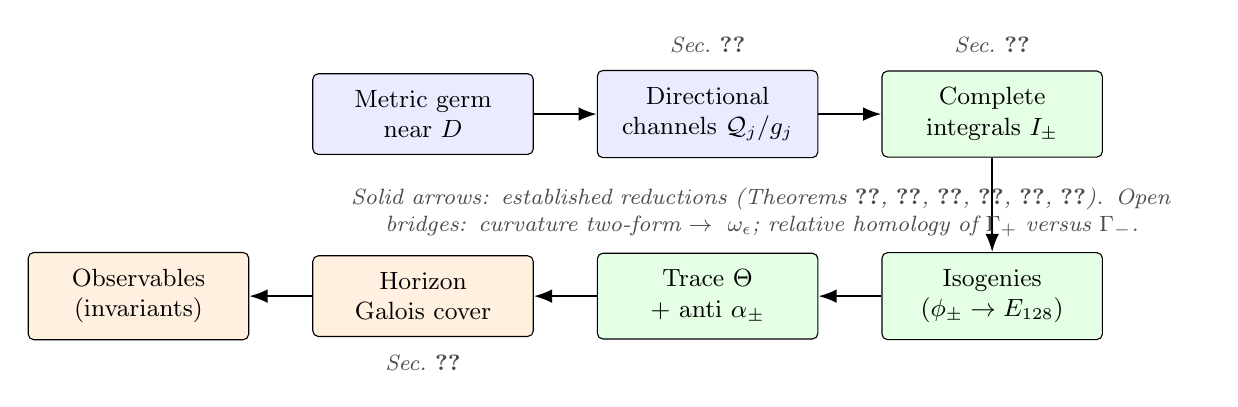
\begin{tikzpicture}[
  font=\small,
  node distance=6mm and 8mm,
  box/.style={draw, rounded corners=2pt, align=center, inner sep=6pt,
              minimum height=10mm, minimum width=28mm},
  arr/.style={-{Latex}, thick},
  note/.style={font=\footnotesize\itshape, text=black!70, align=center}
]
\node[box, fill=blue!8] (germ) {Metric germ\\near \(D\)};
\node[box, fill=blue!8, right=of germ] (chan) {Directional\\channels \(\mathcal Q_j/g_j\)};
\node[box, fill=green!10, right=of chan] (int) {Complete\\integrals \(I_\pm\)};
\node[box, fill=green!10, below=12mm of int] (iso) {Isogenies\\(\(\phi_\pm\to E_{128}\))};
\node[box, fill=green!10, left=of iso] (split) {Trace \(\Theta\)\\+ anti \(\alpha_\pm\)};
\node[box, fill=orange!12, left=of split] (gal) {Horizon\\Galois cover};
\node[box, fill=orange!12, left=of gal] (obs) {Observables\\(invariants)};

\draw[arr] (germ) -- (chan);
\draw[arr] (chan) -- (int);
\draw[arr] (int) -- (iso);
\draw[arr] (iso) -- (split);
\draw[arr] (split) -- (gal);
\draw[arr] (gal) -- (obs);

\node[note, above=1mm of chan] {Sec.~\ref{sec:local}};
\node[note, above=1mm of int] {Sec.~\ref{sec:periods}};
\node[note, below=1mm of gal] {Sec.~\ref{sec:galois}};

\node[note, below=3mm of germ.south west, anchor=north west, text width=0.92\textwidth]
{Solid arrows: established reductions (Theorems~\ref{thm:localdecomp},
\ref{thm:trace}, \ref{thm:anti}, \ref{thm:S5}, \ref{thm:crown20},
\ref{thm:rotwreath}). Open bridges: curvature two-form \(\to\omega_\epsilon\);
relative homology of \(\Gamma_+\) versus \(\Gamma_-\).};
\end{tikzpicture}
\caption{Sequential pipeline of the paper. Each solid arrow is a theorem of
Sections~\ref{sec:local}--\ref{sec:galois}; the two open bridges are stated as
such in the text.}
\label{fig:pipeline}
\end{figure}

Three structural analogies organise the dictionary.

\paragraph{Channel versus sheet.}
Locally, curvature is a sum of directional channels \eqref{eq:Rchannel}. At the
period scale each complementary differential splits as
\eqref{eq:master-split} into a descended trace and an elementary anti term.
Globally, the entropy pair splits into an even sector \(S_L\) and an odd sector
\(S_R\). In every case one decomposes, pushes the even part down, and retains
the odd part as monodromy or path data.

\paragraph{Valuation parity versus Galois parity.}
The master quadric \(C_a(P)\) is a quadratic form on one column of the metric
valuation matrix. Kummer independence is a parity matrix of divisorial
valuations. Both convert a geometric configuration into a linear-algebraic
rank computation.

\paragraph{Cancellation versus completion.}
Theorem~\ref{thm:cancelhier} lists the four ways a local pole order can drop.
Section~\ref{sec:periods} separates completed channel reductions from the open
comparison of \(\Gamma_+\) with \(\Gamma_-\). Theorem~\ref{thm:entropy} separates
certified non-radicality from uncertified inheritance for sector temperatures.
In each case the paper records exact closure status rather than silent
over-claim.

The two open interface theorems are therefore not failures of the spine but
its boundary:
\begin{enumerate}
\item deriving \(\omega_\epsilon\) from the original surface curvature two-form
and matching poles to the local face table;
\item comparing the relative homology classes of \(\Gamma_+\) and \(\Gamma_-\)
on \(E_{128}\).
\end{enumerate}

% =====================================================================
\section{Discussion and open problems}
\label{sec:discussion}
% =====================================================================

The multi-horizon story, read at three scales, is a single even/odd principle.
Locally, pole orders and master coefficients descend as scalar invariants while
individual curvature channels remain chart-dependent. At the period scale, the
even combination of complementary differentials descends to a non-torsion form
\(\Theta\) on \(E_{128}\), while the odd combination is elementary. Globally,
area products, wall data, and left-sector half-energy descend to the
observables, while individual entropies and the sign of \(\vartheta=ST\) live
only on the cover. At four charges a non-solvable wall separates the two
layers: the solution-generating map is radical-one-way.

The classical checks of the hidden-conformal programme are reproduced by the
Galois grading alone, with no conformal input. Those checks therefore carry no
discriminating power about the existence of a dual CFT; the burden of evidence
rests on genuinely quantum observables.

The decorated arithmetic cover is now closed as a degree-\(20\) crown with full
\(C_2^2\wrp S_5\) normal closure, and rotation supplies a controlled third
Kummer channel. Open problems lie higher in the tower or on the two bridges
already named:
\begin{enumerate}
\item extend contact-parity realisation and maximal wreath theorems to every
charge number with known base monodromy;
\item determine the lower symmetric functions of the mass fiber;
\item certify sector-temperature fields;
\item interpret Kummer characters and inertia colours microscopically;
\item classify compactified higher-collision strata;
\item treat five-dimensional and cosmological-constant families;
\item derive \(\omega_\epsilon\) from the surface curvature two-form and match
to Section~\ref{sec:local};
\item compare \(\Gamma_+\) and \(\Gamma_-\) in the relative homology of
\((E_{128},\{P,-P\})\).
\end{enumerate}

% =====================================================================
\appendix
\section{Computational certificates}
\label{app:certs}
% =====================================================================

All machine-checked claims are exact: rational arithmetic in the Python
standard library, symbolic identities in \texttt{sympy}, or Macaulay2 primary
decompositions. Numerics appear only as scaffolding and are discharged by exact
polynomial identities.

{\small
\begin{center}
\begin{tabular}{@{}llp{0.48\textwidth}@{}}
\toprule
Script & Layer & Contents\\
\midrule
\texttt{verify\_local\_curvature\_calculus.py}
  & local
  & \(75\) rational two-jet checks of \eqref{eq:Rchannel}; face laws;
    pure models; KN coefficients\\
\texttt{verify\_dbp\_landen\_trace\_theorem\_v1\_1.py}
  & periods
  & \(75\) exact gates: isogeny, trace, anti, residues, non-torsion\\
\texttt{four\_charge\_crown.py}
  & Galois
  & Prop.~\ref{prop:crown}; anchors\\
\texttt{abel\_ruffini\_black\_holes.py}
  & Galois
  & Thm.~\ref{thm:S5}; Dedekind witnesses\\
\texttt{entropy\_sum\_resolvent.py}
  & Galois
  & Lem.~\ref{lem:collapse}; Thm.~\ref{thm:entropy}\\
\texttt{horizon\_wreath\_inertia\_model.m2}
  & Galois
  & realisation poset; primality of \(I_Z\)\\
\bottomrule
\end{tabular}
\end{center}
}

\paragraph{Dedekind witnesses (Theorem~\ref{thm:S5}).}
Point A: \(M=3\), \(Q=(\tfrac13,\tfrac12,\tfrac25,\tfrac37)\); witness \(p=53\),
type \((2,3)\). Point B: \(M=15\), \(Q=(1,2,3,5)\); witness \(p=23\). Point C:
\(M=2\), \(Q=(\tfrac27,\tfrac59,\tfrac14,\tfrac4{11})\); witness \(p=31\). All
quintics separable and totally real.

\paragraph{Entropy resolvent (Theorem~\ref{thm:entropy}, point B).}
Exact certificates modulo \(\mathcal N\): \(g_i^2\equiv u+N_i^2\),
\(\sum g_i\equiv4M\), \(\alpha^2-u\beta^2\equiv(\prod N_i)^2\). Resolvent
witnesses \(p=17,19,23\), all type \((2,3)\); degree-\(10\) polynomial for
\(S_++S_-\) irreducible over \(\Q\).

\paragraph{Macaulay2.}
Under Macaulay2 1.25.11: \(\operatorname{codim}I_X=5\), relative Jacobian
\(8e_3(w)\), and both \texttt{minimalPrimes IZ} and
\texttt{primaryDecomposition IZ} return the single prime \(I_Z\) of degree
\(64\).

\section{Degree count}
\label{app:degree}

For large \(u\) each factor of \eqref{eq:norm} behaves as
\(4M-(\sum_i\varepsilon_i)\sqrt u+O(u^{-1/2})\). Pairing \(\varepsilon\) with
\(-\varepsilon\): the aligned pair contributes degree \(1\), the four pairs with
\(|\sum\varepsilon|=2\) contribute degree \(4\), and the balanced pairs
contribute degree \(0\) in \(u\). Hence \(\deg_u\mathcal N=5\) and
\(\mathrm{lc}=(-16)(-4)^4(4M)^6=-2^{24}M^6\). The same count gives degrees
\(1,1,4\) at \(n=1,2,3\) charges.

\section{Local computation recipe}
\label{app:recipe}

Given diagonal components \(g_i\), valuation matrix \(P\), and unit/front germs:
verify positivity; form channels \(\mathcal Q_j\); apply \eqref{eq:decomp};
evaluate \(C_a(P)/h_a\); combine equal exponents; inspect inward jets only if an
outer coefficient vanishes; select the Newton face; evaluate the front
coefficient at the declared ratio; report pole order and leading coefficient.
Numerical curvature is a consistency check, not the source of the valuation.

\section{Reproducibility record}
\label{app:repro}

\begin{center}
\begin{tabular}{@{}ll@{}}
\toprule
Item & Record\\
\midrule
Document & v2.1 (13 July 2026), sequential unified preprint\\
Author & William Lloyd\\
Mathematical sources & local curvature calculus v1.0; DBP Landen--Trace v1.1;
  Galois horizon cover v1.0\\
Presentation & rewritten as one narrative (not a verbatim merge)\\
Notation & \(\Theta\): DBP trace on \(E_{128}\); \(\vartheta=ST\): Galois-odd;
  \(\mathcal D\): local transverse drift\\
Curvature convention & unit \(S^2\) has \(R=+2\)\\
Units & \(G=\hbar=c=1\), \(S=A/4\)\\
\bottomrule
\end{tabular}
\end{center}

% =====================================================================
\begin{thebibliography}{99}
\bibitem{CL1} M.~Cveti\v{c} and F.~Larsen,
``General rotating black holes in string theory: Greybody factors and event
horizons,'' Phys.\ Rev.\ D {\bf 56} (1997) 4994, [hep-th/9705192].
\bibitem{CL2} M.~Cveti\v{c} and F.~Larsen,
``Greybody factors for rotating black holes in four dimensions,''
Nucl.\ Phys.\ B {\bf 506} (1997) 107, [hep-th/9706071].
\bibitem{CGLP2018} M.~Cveti\v{c}, G.\,W.~Gibbons, H.~L\"u and C.\,N.~Pope,
``Killing Horizons: Negative Temperatures and Entropy Super-Additivity,''
Phys.\ Rev.\ D {\bf 98} (2018) 106015, [arXiv:1806.11134].
\bibitem{AH} M.~Ansorg and J.~Hennig,
``The inner Cauchy horizon of axisymmetric and stationary black holes with
surrounding matter,'' Class.\ Quant.\ Grav.\ {\bf 25} (2008) 222001,
[arXiv:0810.3998]; Phys.\ Rev.\ Lett.\ {\bf 102} (2009) 221102,
[arXiv:0903.5405].
\bibitem{CGP2011} M.~Cveti\v{c}, G.\,W.~Gibbons and C.\,N.~Pope,
``Universal Area Product Formulae for Rotating and Charged Black Holes in
Four and Higher Dimensions,'' Phys.\ Rev.\ Lett.\ {\bf 106} (2011) 121301,
[arXiv:1011.0008].
\bibitem{CR2012} A.~Castro and M.\,J.~Rodriguez,
``Universal properties and the first law of black hole inner mechanics,''
Phys.\ Rev.\ D {\bf 86} (2012) 024008, [arXiv:1204.1284].
\bibitem{CMS} A.~Castro, A.~Maloney and A.~Strominger,
``Hidden Conformal Symmetry of the Kerr Black Hole,''
Phys.\ Rev.\ D {\bf 82} (2010) 024008, [arXiv:1004.0996].
\bibitem{WangLiu} Y.-Q.~Wang and Y.-X.~Liu,
``Hidden Conformal Symmetry of the Kerr-Newman Black Hole,''
JHEP {\bf 08} (2010) 087, [arXiv:1004.4661].
\bibitem{ChenLong4Q} K.-N.~Shao and Z.~Zhang,
``Hidden Conformal Symmetry of Rotating Black Hole with four Charges,''
Phys.\ Rev.\ D {\bf 83} (2011) 106008, [arXiv:1008.0585].
\bibitem{GHSS} M.~Guica, T.~Hartman, W.~Song and A.~Strominger,
``The Kerr/CFT Correspondence,''
Phys.\ Rev.\ D {\bf 80} (2009) 124008, [arXiv:0809.4266].
\bibitem{CY} M.~Cveti\v{c} and D.~Youm,
``Entropy of non-extreme charged rotating black holes in string theory,''
Phys.\ Rev.\ D {\bf 54} (1996) 2612, [hep-th/9603147].
\bibitem{Std4Q} Z.-W.~Chong, M.~Cveti\v{c}, H.~L\"u and C.\,N.~Pope,
``Charged rotating black holes in four-dimensional gauged and ungauged
supergravities,'' Nucl.\ Phys.\ B {\bf 717} (2005) 246, [hep-th/0411045];
cf.\ also arXiv:1912.08988.
\bibitem{SV} A.~Strominger and C.~Vafa,
``Microscopic origin of the Bekenstein-Hawking entropy,''
Phys.\ Lett.\ B {\bf 379} (1996) 99, [hep-th/9601029].
\bibitem{Moore} G.\,W.~Moore, ``Arithmetic and Attractors,''
[hep-th/9807087].
\bibitem{BKO} N.~Benjamin, S.~Kachru, K.~Ono and L.~Rolen,
``Black holes and class groups,'' Res.\ Math.\ Sci.\ (2018),
[arXiv:1807.00797]; M.~G\"unaydin, S.~Kachru and A.~Tripathy,
[arXiv:1903.02323].
\bibitem{Twofold} C.-M.~Chen, Y.-M.~Huang, J.-R.~Sun, M.-F.~Wu and S.-J.~Zou,
``Twofold Hidden Conformal Symmetries of the Kerr-Newman Black Hole,''
Phys.\ Rev.\ D {\bf 82} (2010) 066004, [arXiv:1006.4097].
\bibitem{Dummit} D.\,S.~Dummit, ``Solving solvable quintics,''
Math.\ Comp.\ {\bf 57} (1991) 387.
\bibitem{M2} D.~R.~Grayson and M.~E.~Stillman,
``Macaulay2,'' \url{https://macaulay2.com/}.
\end{thebibliography}

\end{document}
